\documentclass[usenames,dvipsnames]{beamer}
%
% Choose how your presentation looks.
%
\usepackage[T1]{fontenc}
\usepackage[utf8]{inputenc}
\usepackage{lmodern}  
\usepackage{tikz}%boxy  
\usetikzlibrary{shapes,snakes}
\usetikzlibrary{arrows,positioning}
\usetikzlibrary{calc}
\usepackage{amsmath}
\usepackage{bm}
\usepackage{graphicx}
\usepackage{color}
\usepackage{hyperref}
\usepackage{lipsum}
\usepackage{enumerate}
\usepackage{booktabs}
\usepackage{multirow}
%
% For more themes, color themes and font themes, see:
% http://deic.uab.es/~iblanes/beamer_gallery/index_by_theme.html
%
\mode<presentation>
{
  \usetheme{Darmstadt}      % or try Darmstadt, Madrid, Warsaw, ...
  \usecolortheme{default} % or try albatross, beaver, crane, ...
  \usefonttheme{serif}  % or try default, serif, structurebold, ...
  \setbeamertemplate{navigation symbols}{}
  \setbeamertemplate{caption}[numbered]
  \setbeamertemplate{headline}{}
}
%
% 
%
\newcommand{\mytikzmark}[2]{%
  \tikz[remember picture,inner sep=0pt,outer sep=0pt,baseline,anchor=base] 
    \node (#1) {\ensuremath{#2}};}
%
%
\newcommand*\circled[1]{\tikz[baseline=(char.base)]{
    \node[shape=circle,draw=Red, dashed, inner sep=1pt] (char) {#1};}}
%
\newcommand*\circledd[1]{\tikz[baseline=(char.base)]{
    \node[shape=ellipse,draw=Red, semithick, inner sep=0.2pt] (char) {#1};}}
%
\newcommand*\circleZ[1]{\tikz[baseline=(char.base)]{
    \node[shape=ellipse,draw=Green, semithick, inner sep=0.2pt] (char) {#1};}}
%
\newcommand*{\boxcolor}{Red}
\makeatletter
\renewcommand{\boxed}[1]{\textcolor{\boxcolor}{%
\tikz[baseline={([yshift=-1ex]current bounding box.center)}] \node [rectangle, thick, minimum width=4ex,draw, dashed] {\normalcolor\m@th$\displaystyle#1$};}}
 \makeatother
%
\newcommand*\boxedd[1]{\tikz[baseline=(char.base)]{
    \node[shape=rectangle,draw=Red, semithick, inner sep=2pt] (char) {#1};}}
%
%\newcommand\textbox[1]{%
%  \parbox{.5\textwidth}{#1}%
%}
%
%
\newcommand{\Duck}[1]{\underset{#1}{\max}}
%
%
%
\title[Block 6]{Block 6\\ Limited dependent variables\\(repetition from BSc. courses)}
\author{Advanced econometrics 1 4EK608 \\Pokročilá ekonometrie 1 4EK416}
\institute{Vysoká škola ekonomická v Praze}
\date{}
%
%
%
\begin{document}

\setbeamertemplate{caption}{\raggedright\insertcaption\par}
 
\begin{frame}
  \titlepage
\end{frame}

% Uncomment these lines for an automatically generated outline.
\begin{frame}{Content}
  \tableofcontents
\end{frame}

%---------------------------------
\section{Binary LDVs}
\begin{frame}{Binary dependent variables: LPM, Logit, Probit}
Binary dependent variables: $y_i \in \{0;1\}$\\
\vspace{1cm}
\underline{Linear probabilistic model (LPM) – quick repetition}\\
\bigskip
\begin{itemize}
\item[\checkmark] Simple estimation through OLS \\ easy $\beta_j$-parameter interpretation\\
\medskip
\item[!] $\hat{y}_i$ may get beyond the interpretable $\langle 0, 1 \rangle$ probabilistic interval\\
\smallskip
\item[!] Marginal (partial) effects of the regressors are constant. \\
\smallskip
\item[!] heteroscedastic error term: $\hat{u}_i \sim Bi (0, [\hat{y}_i (1 - \hat{y}_i)])$
\end{itemize}
\end{frame}
%---------------------------------
\begin{frame}{Binary dependent variables: LPM, Logit, Probit}
Binary dependent variables: Logit and Probit\\
\bigskip
{\small
$\mytikzmark{a}{P}(y=1|\bm{x}) = \mytikzmark{b}{G}(\beta_0 + \beta_1 x_1 + \dots + \beta_k x_k) = G(\mytikzmark{c}{\bm{x^{'} \! \beta}})=G(z);$~$0 \!< \!G(z) \!< \! 1$} \\
\vspace*{17mm}
\underline{Cumulative distribution functions (CDFs) for Logit and Probit}\\
\bigskip
{\small
\textcolor{Blue}{Logit: } $G(z) = \Lambda(z) = \exp(z)/[1+\exp(z)]$\\
\bigskip
\textcolor{Blue}{Probit:} $G(z) = \Phi(z) = \int_{-\infty}^{z} \phi(v) dv$; \quad $\phi(z) = (2 \pi)^{-1/2} \exp(-z^2/2)$}
\begin{tikzpicture}[<-,overlay,remember picture,inner sep=1.5pt,shorten <=0.2em,font=\footnotesize]
\tikzset{
    mynode/.style={rectangle, text width=1cm},
    myarrow/.style={->, >=stealth, thin, Red}
}
\node[mynode] at (-10.5,3.1) (A){``Success'' \\ probability};
\node[mynode] at (-2.9,3) (C){Simplified \\ notation};
\draw[myarrow] (A) -- ++ (a);
\draw[myarrow] (C) -- ++ (c);
\tikzset{
    mynode/.style={rectangle, text width=2.5cm},
    myarrow/.style={->, >=stealth, thin, Red}
}
\node[mynode] at (-7.5,2.9) (B){CDF: function of \\ regressor and the \\ $\beta$-parameters};
\draw[myarrow] (B) -- ++ (b);
\end{tikzpicture}
\end{frame}
%---------------------------------
\begin{frame}{Logit vs Probit}
\textcolor{Blue}{Logit: } $G(z) = \Lambda(z) = \exp(z)/[1+\exp(z)]$\\
\bigskip
\textcolor{Blue}{Probit:} $G(z) = \Phi(z) = \int_{-\infty}^{z} \phi(v) dv$\\
\medskip
\begin{minipage}[t]{.6\textwidth}
\begin{figure}
\centering
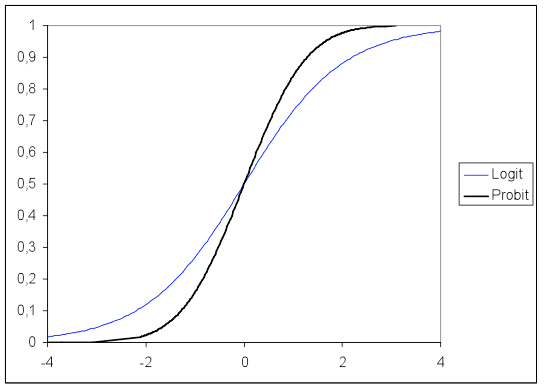
\includegraphics[width=\textwidth]{./img/P11_1}
\end{figure}
\end{minipage}%
\hspace*{7mm}
\begin{minipage}[t]{.3\textwidth}
\begin{flalign*}
G(z_i & = -\infty) & = 0  \\
G(z_i & = ~~0) & = 0.5  \\
G(z_i & = + \infty) & = 1 
\end{flalign*}
\end{minipage}
\end{frame}
%---------------------------------
\begin{frame}{Logit vs Probit}
\begin{itemize}
\item There are no convincing arguments to prefer one model type over the other.
\medskip
\item Logit is used more often, partly due to simpler estimate calculation.
\medskip
\item In economics, we often assume normal distribution of variables, which would imply the use of Probit.
\medskip
\item With Probit, $\beta_j$ parameters have no interpretation \\except for their signs and significance levels. \\ \smallskip (Logit parameters discussed next.)
\end{itemize}
\end{frame}
%---------------------------------
\begin{frame}{Logit – interpretation of model coefficients $\beta$}
$\circled{$P_i $} = P(y_i = 1|\bm{x}_i) = \hat{y}_i = G(\bm{x}_i \bm{\beta}) = G(z)= \circled{$\frac{e^z}{1+e^z}$}$, also:\\
\medskip
$\frac{P_i}{1-P_i}$  \quad is the relative chance of success: \textbf{Odds ratio}\\
\bigskip
\begin{itemize}
\item[] Example: 
\item[] $P_i = 0.8 \leftrightarrow (1-P_i) = 0.2$
\item[] Odds ratio: $\frac{0.8}{0.2} = \frac{4}{1}$
\item[] Interpetation: the relative chance of success is 4 to 1.
\end{itemize}
\end{frame}
%---------------------------------
\begin{frame}{Logit – interpretation of model coefficents $\beta$}
\begin{itemize}
\item $P_i = \frac{e^z}{1+e^z}$ \\
\medskip
\item $1-P_i = 1 - \frac{e^z}{1+e^z} = \frac{(1+e^z) - e^z}{1 + e^z} = \frac{1}{1 + e^z}$\\
\medskip
\item $\frac{P_i}{1-P_i} = \frac{\frac{e^z}{1+e^z}}{\frac{1}{1+e^z}} = e^z$\\
\medskip
\item $\frac{P_i}{1-P_i} = e^z = e^{(\beta_0 + \beta_1 x_1 + \beta_2 x_2 + \dots)}$\\
\medskip
\item $\log(\frac{P_i}{1-P_i}) = \beta_0 + \beta_1 x_1 + \beta_2 x_2 + \dots$\\
\medskip
\item $\beta$ coefficients have a linear interpretation towards the logarithm of relative chance of success (log-odds) \dots \\Also, $\hat{\beta}_j \approx (\% \Delta) \frac{P_i}{1-P_i}$.
\end{itemize}
\end{frame}
%---------------------------------
\begin{frame}{Logit and Probit – estimation}
Density function of $y_i$ (given $x_i$, assuming random sampling):\\
\vspace{0.2cm}
$f(y_i | \bm{x}_i; \bm{\beta}) = [G(\bm{x}_i \bm{\beta})]^{y_i} [1-G(\bm{x}_i \bm{\beta})]^{1-y_i}$\\ 
\vspace{0.2cm}
\textcolor{Green}{\textbf{Maximum Likelihood Estimation (MLE)}} 
\\is used to estimate coefficients $\hat{\bm{\beta}}$. \\
\vspace{0.2cm}
Computers and iterative methods are used to maximize:\\
\bigskip
$LL(\hat{\bm{\beta}}) = \Duck{\bm{\beta}} \{ \sum_{i=1}^N (y_i \log[G(\bm{x}_i \bm{\beta})] + (1-y_i) \log[1-G(\bm{x}_i \bm{\beta})]) \}$,\\
\bigskip
where $LL(\hat{\bm{\beta}})$ is the maximized log-likelihood function, \\
\smallskip
\hspace*{1cm} $G(\cdot)$ is the CDF for Logit or Probit,\\
\smallskip
\hspace*{1cm} $y_i = \{0;1\}$
\end{frame}
%---------------------------------
\begin{frame}{Logit and Probit – estimation}
Example: Married women's labor force participation\\
\bigskip
\begin{minipage}[t]{.6\textwidth}
\begin{table}[]
\resizebox{\textwidth}{!}{%
\begin{tabular}{|l|c|c|c|}
\hline
\multicolumn{4}{|c|}{\textbf{Dependent Variable: \textit{inlf}}}                                                                                                                                             \\ \hline
\textbf{\begin{tabular}[c]{@{}l@{}}Independent \\ Variables\end{tabular}} & \multicolumn{1}{l|}{\textbf{LPM (OLS)}} & \multicolumn{1}{l|}{\textbf{Logit (MLE)}} & \multicolumn{1}{l|}{\textbf{Probit (MLE)}} \\ \hline
\textit{nwifeinc}                                                         & $\underset{(.0015)}{-.0034}$            & $\underset{(.008)}{-.021}$                & $\underset{(.005)}{-.012}$                 \\ \hline
\textit{educ}                                                             & $\underset{(.007)}{.038}$               & $\underset{(.043)}{.221}$                 & $\underset{(.025)}{.131}$                  \\ \hline
\textit{exper}                                                            & $\underset{(.006)}{.039}$               & $\underset{(.032)}{.206}$                 & $\underset{(.019)}{.123}$                  \\ \hline
\textit{$\textit{exper}^2$}                                               & $\underset{(.00018)}{-.00060}$          & $\underset{(.0010)}{-.0032}$              & $\underset{(.0006)}{-.0019}$               \\ \hline
\textit{age}                                                              & $\underset{(.002)}{-.016}$              & $\underset{(.015)}{-.088}$                & $\underset{(.008)}{-.053}$                 \\ \hline
\textit{kidslt6}                                                          & $\underset{(.032)}{-.262}$              & $\underset{(.204)}{-1.443}$               & $\underset{(.119)}{-.868}$                 \\ \hline
\textit{kidsge6}                                                          & $\underset{(.013)}{.013}$               & $\underset{(.075)}{.060}$                 & $\underset{(.043)}{.036}$                  \\ \hline
\textit{constant}                                                         & $\underset{(.151)}{.586}$               & $\underset{(.860)}{.425}$                 & $\underset{(.509)}{.270}$                  \\ \hline
\begin{tabular}[c]{@{}l@{}}Percentage correctly \\ predicted\end{tabular} & 73.4                                    & 73.6                                      & 73.4                                       \\ \hline
Log-likelihood value                                                      & —                                       & -401.77                                   & -401.30                                    \\ \hline
Pseudo \textit{R}-squared                                                 & .264                                    & .220                                      & .221                                       \\ \hline
\end{tabular}%
}
\end{table}
\end{minipage}
\hspace*{1mm}
\begin{minipage}[t]{.35\textwidth}
{\tiny
Coefficients are not comparable across models\\

Often, Logit estimated coefficients $\approx 1.6$ times Probit estimated because $g_{\textit{Logit}}(0) / g_{\textit{Probit}}(0) \approx 1/1.6$.\\

The biggest difference between the LPM and Logit/Probit is that partial effects are nonconstant in Logit/Probit:
\begin{flalign*}
\hat{P}(\textit{working} | \overline{\bm{x}}, \textit{kidslt}6 = 0 ) = .707 && \\
\hat{P}(\textit{working} | \overline{\bm{x}}, \textit{kidslt}6 = 1 ) = .373 && \\
\hat{P}(\textit{working} | \overline{\bm{x}}, \textit{kidslt}6 = 2 ) = .117 && 
\end{flalign*}
\vspace*{-2mm}
(Larger decrease in probability for the first child)}
\end{minipage}
\end{frame}
%---------------------------------
\begin{frame}{Logit and Probit – estimation}
Given random sampling, MLE is consistent, asymptotically efficient and asymptotically normal estimation function.\\ 
\medskip
Asymptotic variances / standard errors can be used to test hypotheses such as $H_0: \beta_j = 0$. \\
\vspace*{1.8cm}
Multiple (compound) hypotheses may be tested using the \textbf{Likelihood ratio} statistics:\\
\medskip
$LR = 2 (\log L_{ur} - \log L_r) \sim \chi_q^2$\\
\medskip
where $L_{ur}$ is the $LL(\hat{\bm{\beta}})$ of the unrestricted ($ur$) model \\
\smallskip
\hspace*{1cm} $L_r$ is the $LL(\hat{\bm{\beta}})$ of the restricted ($r$) model \\
\smallskip
\hspace*{1cm} $q$ is the number of restrictions imposed.
\begin{tikzpicture}[<-,overlay,remember picture,inner sep=1.5pt,shorten <=0.2em,font=\small]
\tikzset{
    mynode/.style={rectangle, draw = Red, text width=3.45cm}
}
\node[mynode] at (0.3,4.3) (A){This is a $ k \times k$ matrix};
\tikzset{
    mynode/.style={rectangle, dashed, very thick, draw=MidnightBlue, fill=ProcessBlue!5, minimum size=1.3cm, text width=5.7cm},
    myarrow/.style={->, >=stealth, thin, Red}
}
\node[mynode] at (-4.9,4.3) (B){$\widehat{\textnormal{Avar}}(\hat{\bm{\beta}}) \equiv \Bigg( \sum \limits_{i=1}^{n} \frac{[g(\bm{x}_i \hat{\bm{\beta}})]^2 \bm{x}_i^{\prime}\bm{x}_i}{G(\bm{x}_i \hat{\bm{\beta}}) [1-G(\bm{x}_i \hat{\bm{\beta}})]} \Bigg)^{-1} $};
\draw[myarrow] (A) -- ++ (B);
\end{tikzpicture}
\end{frame}
%---------------------------------
\begin{frame}{Estimated model and partial/marginal effects}
The effect of a change in $x_j$ on the outcome (probability of success) may be described as follows:\\
\medskip
\begin{itemize}
\item Continuous $x_j$ regressors: \\
\vspace*{4mm}
$\frac{\partial P (y = 1|\bm{x}_i)}{\partial x_j} = g(\bm{x}_i \bm{\beta}) \beta_j$ \quad where \ $g(z) \equiv \frac{dG}{dz}(z)$
\bigskip
\item Binary $x_k$ regressors:
\begin{flalign*}
\Delta P_i = \Delta G(\cdot) & = G(\beta_0 + \beta_1 x_{1,i} + \dots + \beta_{k-1,i} + \beta_k) - && \\
& - G(\beta_0 + \beta_1 x_{1,i} + \dots + \beta_{k-1,i} x_{k-1,i}) &&
\end{flalign*}
\end{itemize}
\medskip
The effect (of a change in $x_{ik}$) differs for each individual (CS unit) $i$  and it is a non-linear function of all parameters from the vector $\bm{\beta}$ and all regressor-values in the row vector $\bm{x}_i$.
\end{frame}
%---------------------------------
\begin{frame}{Estimated model and partial/marginal effects}
Average partial effects (alternatively labelled as marginal effects) are used to summarize the expected effect of a change in a given regressor on the conditional success probability.\\
\bigskip
\textbf{Average Partial Effect (APE):}\\
\medskip
For a binary regressor $x_k$ , we ``simply'' average the individual effects across the whole sample:
\begin{flalign*}
\widehat{\textnormal{APE}}_k & = n^{-1} \sum_{i=1}^N [G(\hat{\beta}_0 + \hat{\beta}_1 x_{1,i} + \dots + \hat{\beta}_{k-1,i} x_{k-1,i} + \hat{\beta}_k ) - && \\
\smallskip
& - G(\hat{\beta}_0 + \hat{\beta}_1 x_{1,i} + \dots + \hat{\beta}_{k-1,i} x_{k-1,i})] &&
\end{flalign*}
For a continuous regressor $x_j$:
\begin{flalign*}
\widehat{\textnormal{APE}}_j = n^{-1} \sum \limits_{i=1}^{n} g(\bm{x}_i \hat{\bm{\beta}}) \hat{\beta}_j &&
\end{flalign*}
\end{frame}
%---------------------------------
\begin{frame}{Estimated model and partial/marginal effects}
\underline{Example: Estimated model (Logit) – APE}\\
\medskip
Wooldridge, MROZ data file, dependent variable: labor force participation of married women.
\begin{flalign*}
\textit{logitmfx} & (\textnormal{formula} = \textit{inlf} \sim \textit{nwifeinc} + \textit{educ} + \textnormal{exper} + \textit{age} + && \\
& + \textit{kidslt}6 + \textit{kidsge}6, \ \textnormal{data} = \textnormal{mroz, atmean} = \textit{F} \ ) && 
\end{flalign*}
\small \qquad Marginal Effects:\\
\vspace{-0.1cm}
\begin{table}[]
\resizebox{.88\textwidth}{!}{%
\begin{tabular}{llllll}
\hline
\multicolumn{1}{c}{} & \multicolumn{1}{c}{$dF/dx$} & \multicolumn{1}{c}{Std. Err.} & \multicolumn{1}{c}{$z$} & \multicolumn{1}{c}{$P>|z|$} & \multicolumn{1}{c}{} \\ \hline
\textit{nwifeinc} & -0.0036634 & 0.0015295 & -2.3951 & 0.01662   & *   \\
\textit{educ}     & ~0.0411306  & 0.0085924 & ~4.7868  & 1.694e-06 & *** \\
\textit{exper}    & ~0.0216992  & 0.0030857 & ~7.0322  & 2.033e-12 & *** \\
\textit{age}      & -0.0165062 & 0.0029573 & -5.5816 & 2.383e-08 & *** \\
\textit{kidslt}6  & -0.2608333 & 0.0428538 & -6.0866 & 1.153e-09 & *** \\
\textit{kidsge}6  & ~0.0105417  & 0.0133312 & 0.7907  & 0.42909   &  \\ \hline
\end{tabular}}
\end{table}
\vspace{-0.1cm}
\small \qquad Signif. codes:  0 `***' 0.001 `**' 0.01 `*' 0.05 `.' 0.1 
\end{frame}
%---------------------------------
\begin{frame}{Estimated model and partial/marginal effects}
As an alternative to APE, we may use average $x_j$  regressor value (sample average) to produce another type of ``summary effect'':\\
\bigskip
\textbf{Partial Effect at the Average (PEA)}\\
\medskip
For any given continuous explanatory variable: $x_j$:
\begin{flalign*}
\widehat{\textnormal{PEA}}_j = g (\overline{\bm{x}}_i \hat{\bm{\beta}}) \hat{\beta}_j &&
\end{flalign*}
For discrete/binary regressors $x_k$, the calculation is analogous.\\
\begin{itemize}
\item[] Warning: 
\\Averaging discrete variables $\Rightarrow$ non-representative values.
\item[] Example: $x_k$ is \textit{female} and we have 47\% of women in the sample. Thus, $\overline{x}_k =0.47$
\end{itemize}
\end{frame}
%---------------------------------
\begin{frame}{Estimated LDV model: evaluation}
$R^2$: not a suitable statistics for the explained variability of  $y_i$. \\
\vspace{0.5cm}
\textbf{McFadden pseudo $\bm{R^2}$}: $\tilde{R}^2 = 1 - \log L_0 / \log L_{ur}$ \\
\medskip
where \qquad $L_0$ is $LL(\hat{\bm{\beta}})$ of the trivial model, often given as:\\ \qquad \qquad \quad $y_i = \beta_0 + u_i$\\

(values such as 0.2 or 0.4 – and higher – are regarded as ``good'')\\
\bigskip
Correct prediction ratio may be calculated based on: 
\vspace*{-2.5mm}
\begin{flalign*}
\tilde{y}_i =
 \begin{cases}
    1 & \ \text{if } G(\bm{x}_i \hat{\bm{\beta}}) > .5 \\
    0 & \ \text{otherwise}
  \end{cases} &&
\end{flalign*}
Correlation between $y_i$ and prediction:\\
\vspace{0.1cm}
$\textit{Corr}(y_i, \tilde{y}_i), \ \textit{Corr}(y_i, G(\bm{x}_i \hat{\bm{\beta}}))$
\end{frame}
%---------------------------------
\begin{frame}{Estimated LDV model: Confusion matrix}
\begin{minipage}[t]{.33\textwidth}
\resizebox{\textwidth}{!}{%
\begin{tabular}{c c | c }
\multicolumn{1}{r}{} &  \multicolumn{1}{c}{\underline{Predicted 1}} & \multicolumn{1}{c}{\underline{Predicted 0}} \\
\rotatebox{90}{\underline{True 1}} & \textcolor{OliveGreen}{\textbf{TP}} & \textcolor{OrangeRed}{\textbf{FN}} \\ 
\cline{2-3}
\rotatebox{90}{\underline{True 0 \ }} & \textcolor{OrangeRed}{\textbf{FP}} & \textcolor{OliveGreen}{\textbf{TN}}
\end{tabular}}
\end{minipage}
\hspace*{-1mm}
\begin{minipage}[t]{.65\textwidth}
\resizebox{\textwidth}{!}{%
\begin{tabular}{c c c | c | c }
& & \multicolumn{2}{ c }{True diagnosis} \\ \cline{3-4}
& & \multicolumn{1}{ |c| }{Positive} & \multicolumn{1}{ c| }{Negative} & \multicolumn{1}{ c }{Total} \\ \cline{2-4}
\multicolumn{1}{ c }{\multirow{2}{*}{Screening test} } & 
\multicolumn{1}{ |c| }{Positive} & $a$ & $b$ & \multicolumn{1}{ |c }{$a+b$} \\ \cline{2-4}
\multicolumn{1}{c}{} &
\multicolumn{1}{ |c| }{Negative} & $c$ & $d$ & \multicolumn{1}{ |c }{$c + d$} \\ \cline{2-4}
& \multicolumn{1}{c}{Total} & \multicolumn{1}{c}{$a+c$} & \multicolumn{1}{c}{$b+d$} & $N$ \\
\end{tabular}}
\end{minipage} \\
\vspace*{1cm}

{\small
$\textit{Accuracy} = \textnormal{(TP + TN)} / N = (a+d)/N$ \\
\vspace*{-6mm}
\begin{flalign*}
\textit{Sensitivity} & = \textit{True positive rate} = \textnormal{TP} / \textit{Actual condition positive} = \\ 
& = \textnormal{TP/(TP+FN)} = a/(a+c)  && \\
\textit{Specificity} & = \textit{True negative rate} = \textnormal{TN}/\textit{Actual condition negative} = \\
& = \textnormal{TN/(FP+TN)} = d/(b+d) &&
\end{flalign*} \\
\vspace*{-2mm}
$\textit{False discovery rate} =\textnormal{ FP/(TP+FP)} = b/(a+b)$ \\
$\textit{Prevalence} = \textit{Condition positive}/N$}
\begin{tikzpicture}[<-,overlay,remember picture,inner sep=1.5pt,shorten <=0.2em,font=\small]
\tikzset{
    mynode/.style={rectangle, draw = Gray, minimum size=2.2cm, text width=3.5cm}
}
\node[mynode] at (-3.6,5.6) (A){};
\tikzset{
    mynode/.style={rectangle, draw = Gray, minimum size=1.83cm, text width=6.8cm}
}
\node[mynode] at (1.8,5.62) (A){};
\end{tikzpicture}
\end{frame}
%---------------------------------
\begin{frame}{Estimated LDV model: Confusion matrix}
\begin{figure}
\centering
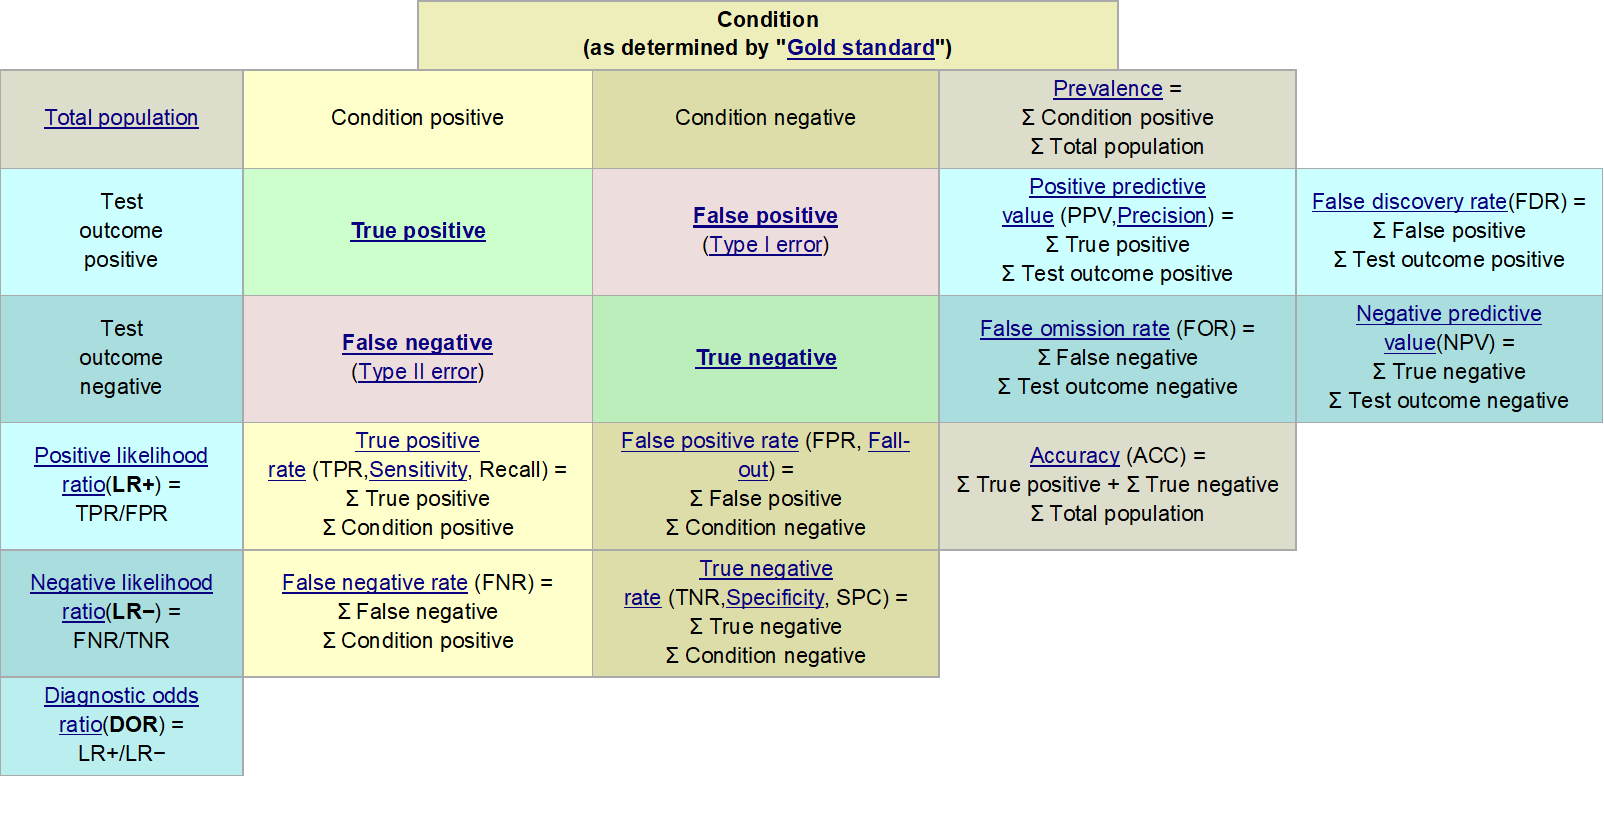
\includegraphics[width=1.06\textwidth]{./img/P11_2}
\end{figure}
\end{frame}
%---------------------------------
\begin{frame}{Estimated LDV model: Accuracy}
\begin{minipage}[c]{.49\textwidth}
\begin{figure}
\centering
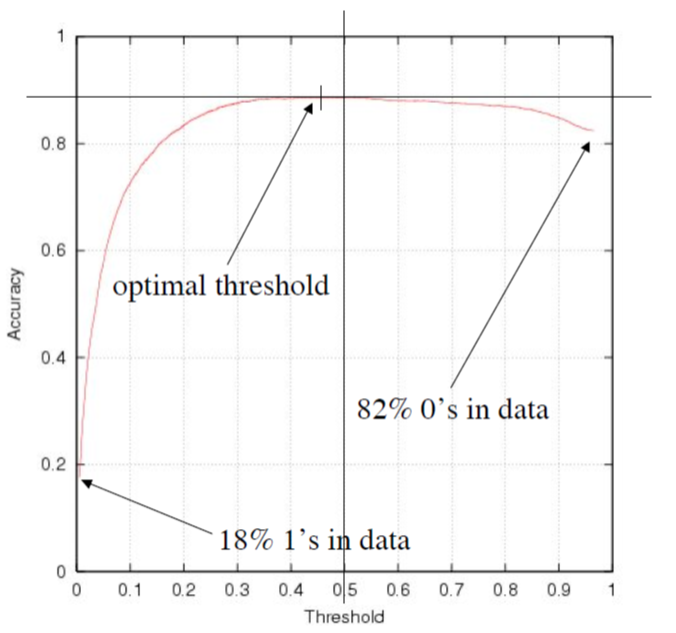
\includegraphics[width=1.06\textwidth]{./img/P11_3}
\end{figure}
\end{minipage}%
\hspace*{5mm}
\begin{minipage}[c]{.49\textwidth}
{\footnotesize
\begin{flalign*}
\tilde{y}_i =
 \begin{cases}
    1 & \ \text{if } G(\bm{x}_i \hat{\bm{\beta}}) \circled{$> .5$} \\
    0 & \ \text{otherwise}
  \end{cases} &&
\end{flalign*}
By changing the  success prediction threshold, we can influence the overal prediction accuracy (classification effectiveness of the model). \\

To maximize \textit{Accuracy}, we can find an optimal ``threshold'' within the $ \langle 0;1 \rangle$ interval. \\
\textbf{Problem}: FP and FN may be associated with different ``costs''. \\
\textbf{Solution}: use weighted statistics or use ROC.}

\end{minipage}
\end{frame}
%---------------------------------
\begin{frame}{Estimated LDV model: ROC curve}
\begin{itemize}
\item Receiver Operator Characteristic (ROC) Curve
\item Developed in WWII to statistically model false positive and false negative detections of radar operators.
\item Suitable for evaluating prediction/classification performance of different models and estimation methods used (Logit, Probit, \dots)
\end{itemize} 
\vspace*{0.5cm}
\quad \textbf{ROC:}\\
\begin{itemize}
\item True Positive Rate vs. False Positive Rate
\item Sensitivity vs. (1 – Specificity)
\end{itemize}
\end{frame}
%---------------------------------
\begin{frame}{Estimated LDV model: ROC curve}
\begin{minipage}[c]{.42\textwidth}
\begin{figure}
\centering
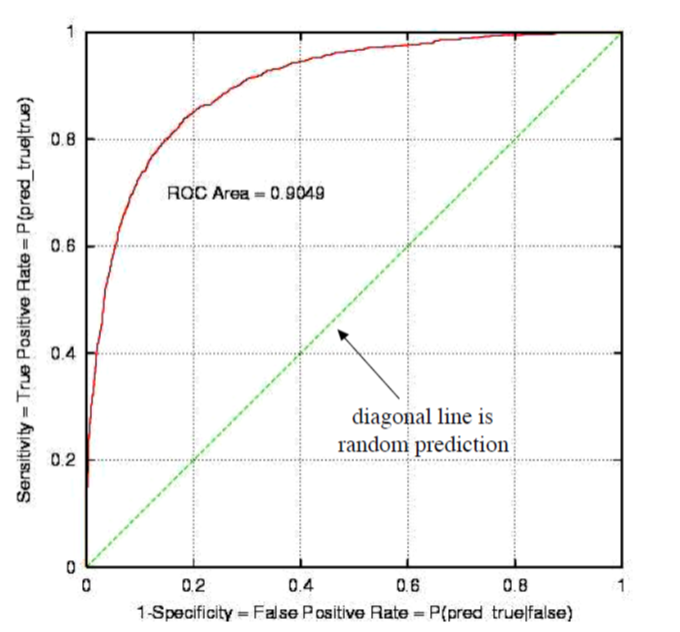
\includegraphics[width=1.25\textwidth]{./img/P11_4}
\end{figure}
\end{minipage}%
\hspace*{8.2mm}
\begin{minipage}[c]{.58\textwidth}
ROC Area – Area under curve (AUC) \\
$1.0$ – perfect prediction \\
$0.9$ – very good prediction \\
$0.6$ – poor prediction \\
$0.5$ – random prediction \\
$< 0.5$ – something is wrong!
\end{minipage}
\end{frame}
%---------------------------------
\begin{frame}{Estimated LDV model: ROC curve}
\begin{itemize}
\item ROC: slope is non-increasing
\item Each point on ROC represents different trade-off \\(cost ratio) between false positives and false negatives
\item AUC (ROC Area) represents model performance averaged over all possible cost ratios 
\item ROC may not be generalized for multinomial models (possible for \textit{Accuracy})
\end{itemize} 
\quad \underline{Comparison and evaluation of ROC curves:}\\
\begin{itemize}
\item If two ROC curves do not intersect, one model (method) dominates the other.
\item If two ROC curves intersect, one model (method) is better for some cost ratios, and other model is better for other cost ratios.
\end{itemize}
\end{frame}
%---------------------------------
\section{Count LDVs}
\begin{frame}{Count dependent variables}
Introduction \\
\bigskip
The dependent variable is a count variable, takes on nonnegative integer values: $\textcolor{Red}{\textbf{0}}, 1,2,3,\dots$ \\
\medskip
\quad {\small Specifically, Poisson regression applies best when $y_i$ takes on \\
\quad relatively few values (including zero).} \\
\bigskip
The count variable describes the number of specific events that occur during a preset period of time. \\
\medskip
Not to be confused with: \\
\begin{itemize}
\item \textcolor{Blue}{Binary data:} $y \in \{0;1\}$
\item \textcolor{Blue}{Ordered multinomial data:} ranking of the observed events is relevant/important.
\end{itemize}
\end{frame}
%---------------------------------
\subsection{Poisson and Negative Binomial}
\begin{frame}{Poisson regression model}
\begin{itemize}
\item Models the relationship between a Poisson-distributed response variable and one or more explanatory variables. \\
\bigskip
\item The explanatory variables can be either continuous, discrete or categorical (factors/dummies). \\
\bigskip
\item The Poisson model predicts the number of occurences of an event with a mean that depends on a set of exogenous regressors $\bm{x}_i$.
\end{itemize}
\end{frame}
%---------------------------------
\begin{frame}{Poisson regression model}
\begin{flalign*}
P(\mytikzmark{y}{y}=h) = \mytikzmark{f}{\exp [-\mu][\mu]^h / h!}, \quad h = 0,1,2, \dots &&
\end{flalign*} \\
\vspace*{1cm}
Model the mean of the dependent variable as a function of explanatory variables:
\begin{flalign*}
\mu(\bm{x}) = \exp(\bm{x \beta}) = \exp (\beta_0 + \beta_1 x_1 + \dots + \beta_k x_k) > 0 &&
\end{flalign*}
The Poisson regression model models a count variable as a function of explanatory variables:
\begin{flalign*}
P(y=h|\bm{x}) = \exp [- \exp(\bm{x \beta})] [\exp(\bm{x \beta})]^h / h!, \quad h = 0,1,2,\dots &&
\end{flalign*}
\begin{tikzpicture}[<-,overlay,remember picture,inner sep=1.5pt,shorten <=0.2em,font=\footnotesize]
\tikzset{
    mynode/.style={rectangle, minimum size=1cm, text width=4.5cm},
    myarrow/.style={->, >=stealth, semithick, Red}
}
\node[mynode] at (2.2,5.4)(box1){Probability that $y$ takes on some integer value of $h$};
\node[mynode] at (7,5.4)(box2){Poisson distribution fuction, where: $\mu = E(y) > 0$};
\draw[myarrow] (box1) -- ++ (y);
\draw[myarrow] (box2) -- ++ (f);
\end{tikzpicture}
\end{frame}
%---------------------------------
\begin{frame}{Poisson regression model}
\begin{flalign*}
P(y=h|\bm{x}) = \exp [- \exp(\bm{x \beta})] [\exp(\bm{x \beta})]^h / h!, \quad h = 0,1,2,\dots &&
\end{flalign*} 
May also be re-written as:
\begin{flalign*}
P(y=h|\bm{x}) = \frac{e^{-\mu} \mu^h}{h!} &&
\end{flalign*} \\
\vspace*{2mm}
where: $\mu = \exp(\bm{x}^{\prime} \bm{\beta})$ \\
\medskip
and $\mu = E(y|\bm{x}) = \textit{var} (y|\bm{x})$
\end{frame}
%---------------------------------
\begin{frame}{Poisson regression model}
\textbf{Interpretation of the coefficients of Poisson regression:}
\begin{flalign*}
\frac{\partial \mu(\bm{x})}{\partial x_j} = \exp (\bm{x \beta})\beta_j = \mu(\bm{x}) \beta_j \Rightarrow \mytikzmark{B}{\boxed{\beta_j = \frac{\frac{\partial \mu(\bm{x})}{\mu(\bm{x})}}{\partial x_j}}} &&
\end{flalign*} 
\vspace{0.5cm}
\underline{\textbf{MLE: ML estimation of the Poisson regression model}}\\
\vspace{-0.4cm}
\begin{flalign*}
\max \log L(\bm{\beta}) = \sum \limits_{i = 1}^{n} \log P(y = y_i | \bm{x}_i) = \sum \limits_{i = 1}^{n} y_i \bm{x}_i \bm{\beta} - \exp (\bm{x}_i \bm{\beta}) &&
\end{flalign*}
A limitation of the model is that it assumes: $E(y|\bm{x}) = \textit{var} (y|\bm{x})$ \\
\medskip
ML estimators in the Poisson regression model are consistent and asymptotically normal even if the Poisson distribution assumption (equidispersion) does not hold.
\begin{tikzpicture}[<-,overlay,remember picture,inner sep=1.5pt,shorten <=0.2em,font=\scriptsize]
\tikzset{
    mynode/.style={rectangle, minimum size=3cm, text width=3.25cm},
    myarrow/.style={->, >=stealth, semithick, Red}
}
\node[mynode] at (2.4,5.70)(box){$(\% \Delta) E(y)$ \dots by what percentage does the mean (expected) outcome change if $x_j$ is \\increased by one?};
\draw[myarrow] (box) -- ++ (B);
\end{tikzpicture}
\end{frame}
%---------------------------------
\begin{frame}{Poisson regression model}
\begin{minipage}[t]{.55\textwidth}
\begin{table}[]
{\tiny
\begin{tabular}{lcc}
\hline
\multicolumn{3}{c}{\textit{\textbf{Dependent Variable: narr86}}}                                                                                                                                              \\ \hline
\multicolumn{1}{c}{\textbf{\begin{tabular}[c]{@{}c@{}}Independent \\ Variables\end{tabular}}} & \textbf{Linear (OLS)}           & \textbf{\begin{tabular}[c]{@{}c@{}}Exponential \\ (Poisson QMLE)\end{tabular}} \\ \hline
\textit{pcnv}                                                                                   & $\underset{(.040)}{-.132}$   & $\underset{(.085)}{-.402}$                                                     \\ \hline
\textit{avgsen}                                                                                 & $\underset{(.012)}{.011}$    & \mytikzmark{sem}{\circledd{$\underset{(.020)}{-.024}$}}                        \\ \hline
\textit{tottime}                                                                                & $\underset{(.009)}{.012}$    & $\underset{(.015)}{.024}$                                                      \\ \hline
\textit{ptime}86                                                                                & $\underset{(.009)}{-.041}$   & $\underset{(.021)}{-.099}$                                                     \\ \hline
\textit{qemp}86                                                                                 & $\underset{(.014)}{-.051}$   & $\underset{(.029)}{-.038}$                                                     \\ \hline
\textit{inc}86                                                                                  & $\underset{(.0003)}{-.0015}$ & $\underset{(.0010)}{-.0081}$                                                   \\ \hline
\textit{black}                                                                                  & $\underset{(.045)}{.327}$    & $\underset{(.074)}{.661}$                                                      \\ \hline
\textit{hispan}                                                                                 & $\underset{(.040)}{.194}$    & $\underset{(.074)}{.500}$                                                      \\ \hline
\textit{born}60                                                                                 & $\underset{(.033)}{-.022}$   & $\underset{(.064)}{-.051}$                                                     \\ \hline
\textit{constant}                                                                               & $\underset{(.038)}{.577}$    & $\underset{(.067)}{-.600}$                                                     \\ \hline
Log-likelihood value                                                                            & —                            & -2,248.76                                                                      \\ 
\textit{R}-squared                                                                              & .073                         & .077                                                                           \\ 
$\hat{\sigma}$                                                                                  & .829                         & 1.232                                                                          \\ 
\end{tabular}}
\end{table}
\end{minipage}
\hspace*{1.3cm}
\begin{minipage}[t]{.3\textwidth}
\vspace*{1.3cm}
{\scriptsize
Wooldridge (crime1) example:\\

\mytikzmark{odsad}{\textnormal{The expected number}} of 1986 arrests falls by 2.4 \% if ``\textit{avgsen}'' increases by one unit (one month).\\

Note the different values and different meanings of the OLS-generated \\ coefficients.}
\end{minipage}
\begin{tikzpicture}[<-,overlay,remember picture,inner sep=1.5pt,shorten <=0.2em,font=\scriptsize]
\tikzset{
    myarrow/.style={->, >=stealth, semithick, Red}
}
\draw[myarrow] (odsad) -- ++ (sem);
\end{tikzpicture}
\end{frame}
%---------------------------------
\begin{frame}{Poisson regression model}
Violation of the \textbf{equidispersion} assumption: {\small $E(y|\bm{x}) = \textit{var} (y|\bm{x})$} \\
\begin{itemize}
\item Often violated in real (economic) data: {\small $E(y|\bm{x}) < \textit{var} (y|\bm{x})$}
\item Most often caused by highly skewed dependent variables. 
\end{itemize}
\bigskip
Impacts of \textbf{overdispersion}:
\begin{itemize}
\item Underestimated standard errors lead to overestimated significance of the estimated parameters.
\item Predicted outcomes (counts / realizations of the dependent variable) are not necessarily skewed.
\end{itemize} 
\end{frame}
%---------------------------------
\begin{frame}{Negative Binomial and Poisson distributions}
\begin{figure}
\centering
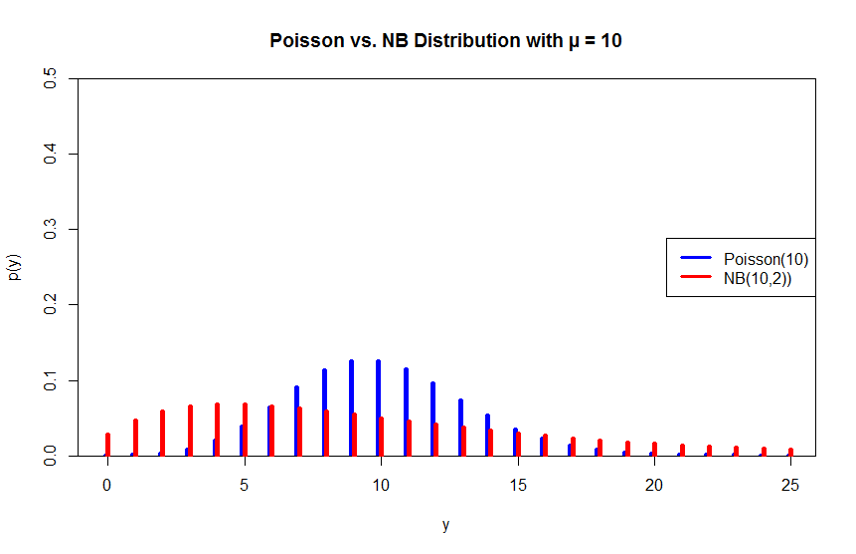
\includegraphics[width=\textwidth]{./img/P11_5}
\end{figure}
\end{frame}
%---------------------------------
\begin{frame}{NB regression model}
\textbf{Overdispersion}\\
\bigskip
Observed variance > theoretical Poisson variance \\
\medskip
$\textit{var} (y) = \mu + \alpha \times f(\mu)$, \quad ($\alpha$: dispersion parameter)\\
\medskip
\begin{itemize}
\item Observed variance \& implications
\vspace{0.3cm}
\begin{itemize}
\item[$\alpha = 0$] Poisson distribution, Poisson model
\vspace{0.2cm}
\item[$\alpha > 0$] Overdispersion (common count variable behavior), \\NB distribution, NB model
\vspace{0.2cm}
\item [$\alpha < 0$]  Underdispersion  (not common)
\end{itemize}
\end{itemize}
\end{frame}
%---------------------------------
\begin{frame}{NB regression model}
\begin{itemize}
\item $y \sim \textnormal{NB}(\mu, \alpha)$\\
\bigskip
\item $\mu = E(y|\bm{x}) = \exp (\bm{x}^{\prime} \bm{\beta})$\\
\bigskip
\item $\alpha$ \dots denotes the dispersion parameter (not variance)\\
\bigskip
\item $\textit{var} (y|\bm{x}) = \mu + \alpha \mu^2$, alternatively $\textit{var} (y|\bm{x}) = \mu + \alpha \mu$
\end{itemize}
\end{frame}
%---------------------------------
\begin{frame}{NB regression model}
Negative binomial distribution can be used to model count data with overdispersion if Poisson model is not suitable ($\alpha > 0$): \\
\bigskip
$$P(Y \!=y|\mu, \alpha) = \frac{\Gamma(y+\alpha^{-1})}{y! \Gamma(\alpha^{-1})} \Big(\frac{\alpha^{-1}}{\alpha^{-1} + \mu}\Big)^{\alpha^{-1}} \! \Big( \frac{\mu}{\alpha^{-1} + \mu} \Big)^{y}, ~~y=0,1,2,\dots$$
\bigskip
where $\Gamma(\cdot)$ is the CDF  for Gamma distr., defined for $r>0$ 
\vspace{-0.3cm}
\\by the following expression: 
$$\Gamma(r) = \int_0^{\infty} z^{r-1} \exp (-z) dz.$$
\medskip
where $\mu_i = \exp (\bm{x}^{\prime} \bm{\beta}) = E(y_i|\bm{x}_i)$
\end{frame}
%---------------------------------
\begin{frame}{Poisson and NB regression models}
\qquad \qquad \qquad \qquad \qquad \qquad \boxedd{$\mu_i = \exp (\bm{x}^{\prime} \bm{\beta}) = E(y|\bm{x}_i)$}\\
~\\
Maximum Likelihood for Poisson regression\\
\vspace{0.3cm}
$LL = \sum \limits_{i = 1}^{n} [-\mu_i + y_i \log(\mu_i) \circledd{$ - \log(y_i!)$}]$\\
\vspace*{1.1cm}
Maximum Likelihood for Negative-Binomial regression\\
\medskip
$LL =  \sum \limits_{i = 1}^{n} \bigg[ \log \bigg( \frac{\Gamma(y+\alpha^{-1})}{y! \Gamma (\alpha^{-1})} \bigg) - (y_i + \alpha^{-1}) \log(1 + \alpha \mu_i) + y_i \log(\alpha \mu_i) \bigg]$
\begin{tikzpicture}[<-,overlay,remember picture,inner sep=1.5pt,shorten <=0.2em,font=\small]
\tikzset{
    mynode/.style={rectangle, Red, minimum size=2.2cm, text width=4.2cm}
}
\node[mynode] at (9.3,3.2) (redtext){This drops out from the $LL$-maximization as its not a function of $\beta$};
\end{tikzpicture}
\end{frame}
%---------------------------------
\begin{frame}{Poisson and NB regression models}
\underline{Estimated parameters: Poisson/NB model}\\
\vspace*{.7cm}
Poisson regression
\begin{itemize}
\item[] $\beta_0, \beta_1, \dots, \beta_k$
\end{itemize}
\bigskip
NB regression
\begin{itemize}
\item[] $\beta_0, \beta_1, \dots, \beta_k$ \textbf{and} $\alpha$
\end{itemize}
\end{frame}
%---------------------------------
\subsection{Zero-Inflated and Hurdle}
\begin{frame}{Zero-inflated and Hurdle models}

{\small
Used to handle the “excess zeroes” issue in the dependent variable. \\
\bigskip
\textbf{Zero-Inflated models:}\\
Instead of assuming that count outcome comes from a single data generating process, we can assume that the count outcome is generated by two systematically different statistical processes:
\begin{itemize}
\item[1.] Logit model \\
(possibility of non-zero outcome is modelled)
\item[2.] Poisson or Negative-Binomial model \\
(model expected outcome for the group where non-zero outcome is assumed possible)
\end{itemize}
\bigskip
\textbf{Hurdle models:}\\
Often used for modelling DGP associated with two-stage decision making: In the first stage, individuals decide on participation (purchasing activity) and in the second stage, they decide upon intensity (how many ``items'' are purchased).
}
\end{frame}
%---------------------------------
\begin{frame}{Zero-inflated and Hurdle models}
\begin{minipage}[t]{.49\textwidth}
\underline{\textbf{ZI models}} \\

\small{Ex.1: Internet usage at work\\
We model hours spent on the internet per day\\
Some people don't have internet at work.\\
For those who have, Poiss/NB is used.\\
~\\
Ex.2: Marathons per year\\
People are/are not active athletes.\\
For athletes, \# marathons is modelled by Poiss/NB.}
\end{minipage}%
\hspace*{7mm}
\begin{minipage}[t]{.49\textwidth}
\underline{\textbf{Hurdle models}} \\

\small{Ex.1: Predict purchased amounts \\
Decision upon purchase.\\
Decision upon (non-zero) amount.\\
~\\
~\\
~\\
~\\
~\\
Ex.2: Doctor visits per year\\
Does the person visit a doctor at all? 
If yes, how may times?\\(You decide on GP ``first'' visit, they may send you to specialists.)}
\end{minipage}
\end{frame}
%---------------------------------
\begin{frame}{Zero-inflated models}
We assume two types of individuals (C-S units) in the sample\\
\begin{itemize}
\item[] \underline{\textbf{Type A:}} Outcome is always zero.\\
Prob($y_i=0) =1$,~~Prob($y_i>0) =0$.\\
\smallskip
\item[] \underline{\textbf{Type non-A:}} Non-zero chance of positive count value. Probability is variable (given regressor values) and follows Poison/NB distributions.
\smallskip
\item[] Binary regime indicator: \\
$z=0$ for type A, $z=1$ for type non-A.
\end{itemize}
\medskip
\small{Prob$(y_i=0|\bm{x}_i) = $ Prob$(z_i\!=\!0)$ +  Prob$(y_i=0|\bm{x}_i, z_i\!=\!1)~\cdot$ Prob$(z_i\!=\!1)$}\\
\small{Prob$(y_i=j|\bm{x}_i) =$ Prob$(y_i=j|\bm{x}_i, z_i\!=\!1)~\cdot$ Prob$(z_i\!=\!1),\quad j=1,2,\dots$}
\end{frame}
%---------------------------------
\begin{frame}{Zero-inflated models}
\small{Prob$(y_i=0|\bm{x}_i) = $ Prob$(z_i\!=\!0)$ +  Prob$(y_i=0|\bm{x}_i, z_i\!=\!1)~\cdot$ Prob$(z_i\!=\!1)$}\\
\small{Prob$(y_i=j|\bm{x}_i) =$ Prob$(y_i=j|\bm{x}_i, z_i\!=\!1)~\cdot$ Prob$(z_i\!=\!1),\quad j=1,2,\dots$}\\
\medskip
May be extended by modelling $z$-regime:
\begin{itemize}
\item[1.] Use logit/probit to model group membership (A vs non-A)
\item[2.] Use Poisson or NB to model counts for the  non-A group\\
\end{itemize}
\medskip
ZI model (Logit/Poisson) example:\\
\medskip
$\textnormal{Prob}(z_i=0|\bm{w}_i) = \frac{\exp(\bm{w}_i^{\prime}\bm{\beta})}{1+\exp(\bm{w}_i^{\prime}\bm{\beta})}$, ~~~~~~~~~~for $z_i = 0$, $y_i$ is always zero.\\
\medskip
$\textnormal{Prob}(y_i=j|\bm{x}_i,z_i\!=\!1) = \frac{\exp(-\lambda_i)\lambda_i^j}{j!}$, ~~~for $z_i = 1$, $y_i$ a count variable.\\
\bigskip
Testing for ZI redundancy ($H_0$ of Poisson vs. $H_1$ ZI Poisson) is non-trivial. The two distributions are different, e.g. $H_0$ and $H_1$ are non-nested. See Greene (ch. 18) and \texttt{R} for available tests.
\end{frame}
%---------------------------------
\begin{frame}{Hurdle models}

Like ZI models, Hurdle count models are two-component models\\
\bigskip
\begin{itemize}
    \item Hurdle component models the zero counts.
    \item Truncated count component for positive counts.
\end{itemize}
\bigskip
\textbf{Unlike ZI models, there is only one source of zeros.}\\
~\\
Count model is only employed if the hurdle for modeling the occurrence of zeros is exceeded. \\
~\\
Count model is typically a truncated Poisson or NB regression
\end{frame}
%---------------------------------
\begin{frame}{Hurdle models}
Hurdle model (Logit/Poisson) example:\\
\bigskip
$\textnormal{Prob}(y_i=0|\bm{w}_i) = \frac{\exp(\bm{w}_i^{\prime}\bm{\beta})}{1+\exp(\bm{w}_i^{\prime}\bm{\beta})} = \Lambda(\bm{w}_i^{\prime}\bm{\beta}) $\\
\bigskip
$\textnormal{Prob}(y_i=j|\bm{x}_i,\bm{w}_i, y_i\!>\!0) = \frac{[1-\Lambda(\bm{w}_i^{\prime}\bm{\beta})]\exp(-\lambda_i)\lambda_i^j}{j![1-\exp(-\lambda_i)]}$.\\
~\\
\bigskip
Again, it is complicated to test for Hurdle model redundancy \\$H_0$ of Poisson vs. $H_1$ Hurdle (say, logit+Poisson) \\
\medskip
The two distributions are non-nested. \\
See Greene (ch. 18) and \texttt{R} for available tests.
\end{frame}
%---------------------------------
\begin{frame}{Count data models in  \texttt{R}}
Poisson model \qquad \qquad R: \{stats\} package\\
\texttt{\textcolor{Green}{glm(y $\sim$ x, family = poisson, \dots )}}\\
\vspace*{.4cm}
NB model \qquad \qquad \qquad R: \{MASS\} package\\
\texttt{\textcolor{Green}{glm.nb(y $\sim$ x, \dots)}} \\
\vspace*{.4cm}
Zero-Inflated model \qquad R: \{pscl\} package\\
\small{\texttt{\textcolor{Green}{zeroinfl(y $\sim$ x|z, link = ``logit'', dist = ``poisson'', \dots)}}} \\
\small{\texttt{\texttt{\textcolor{Green}{zeroinfl(y $\sim$ x|z, link = ``logit'', dist = ``negbin'', \dots)}}}} \\
\qquad $x1+x2$ are the count regressors and $z1+z2$ are regressors of\\ 
\qquad the ZI component. $[$overlap among $x$ and $z$ is possible$]$\\
\vspace*{.4cm}
Hurdle model \qquad \qquad \qquad R: \{pscl\} package\\
\small{\texttt{\textcolor{Green}{hurdle(y $\sim$ x|z, dist=``poisson'', zero.dist=``binomial'' \dots)}}} \\
\qquad $x1+x2$ are the count regressors and $z1+z2$ are regressors of\\ 
\qquad the zero hurdle model. $[$overlap among $x$ and $z$ is possible$]$
\end{frame}
%---------------------------------
\section{Multinomial LDVs}

\subsection{Unordered}

\begin{frame}{Multinomial dependent variables}
\textbf{Introduction} \\
\bigskip
Multinomial dependent variables $\leftrightarrow$ discrete response models for $ > 2$ outcomes\\
\medskip
Two basic types of outcomes / ``choices'' / dependent variables:\\
\bigskip
\textcolor{Blue}{\textbf{Unordered alternatives}} (nominal outcome) \\
\quad Examples: occupational choice, commuting \& transportation\\ \quad choice \dots \\
\medskip
\textcolor{Blue}{\textbf{Ordered alternatives}} (ordered outcome) \\
\quad Examples: Bond ratings, credit ratings \dots
\end{frame}
%---------------------------------
\begin{frame}{Multinomial dependent variables}
\textcolor{Blue}{\textbf{Logit and Probit (MLE for binary dependent variables)}}\\
\begin{itemize}
\item May be extended to cases with more than 2 possible outcomes. \\
\medskip
\item Ordered and unordered outcomes\\
– differ in both model estimation and result interpretation. \\
\vspace{0.8cm}
\item Alternatives (choices, outcomes) for the $i$-th individual: \\$y_i \in \{ 0,1, \dots, J \}$ \\
\vspace{0.3cm}
\dots \quad i.e. $y$ takes on $J+1$ ``values'' 
\\ \qquad (both ordered \& unordered types).
\end{itemize}
\end{frame}
%---------------------------------
\begin{frame}{MDVs: Unordered responses}
$y_i \in \{ 0,1, \dots, J \}$ \\
\vspace{0.2cm}
\textbf{Note:} outcome ordering is arbitrary, as well as the choice of \\the base outcome, i.e. the choice of $i$ where $y_i = 0$. \\
\bigskip
\underline{\textbf{Two basic model-types for unordered responses exist:}} \\
\bigskip
\textcolor{Blue}{Multinomial logit (MNL)} \\
$y$ is an unordered response and we have a set of conditioning variables $\bm{x}$, that change by unit but not by alternative. \\For example, we assume that health-plan choice depends on the age and wage of individuals but not on features (e.g. costs) of alternative health-plans. \\
\medskip
\textcolor{Blue}{Probabilistic choice model (Conditional logit model: CL)} \\
Conditioning variables $\bm{x}$ can change by units and alternatives.\\
Transportation choice: individual's characteristics \& time and cost of travel.
\end{frame}
%---------------------------------
\begin{frame}{MDVs: Multinomial logit (MNL)}
In this model, we are interested in the response (outcome) probabilities: \\
\begin{itemize}
\item[] $p_j (\bm{x}) = P(y= j|\bm{x})$, \qquad $j = 0,1, \dots, J$.
\end{itemize}
\bigskip
Since exactly one choice is possible \\(each individual / CS unit chooses one alternative), \\
\medskip
$p_0 (\bm{x}) + p_1 (\bm{x}) + \dots + p_J (\bm{x}) = 1$ \\
\medskip
allways holds, for all $\bm{x}$.
\end{frame}
%---------------------------------
\begin{frame}{MDVs: Multinomial logit (MNL)}
MNL response probabilities are given as \\
\vspace*{1cm}
$P(y= j|\bm{x}) = \frac{\exp (\bm{x} \bm{\beta}_j) }{[1 + \sum_{h=1}^{J} \exp(\bm{x} \bm{\beta}_h)]}$, \quad $j=1,\dots,J$ \\
\medskip
$P(y= 0|\bm{x}) = \frac{\mytikzmark{1}{\circledd{$1$}}}{[1 + \sum_{h=1}^{J} \exp(\bm{x} \bm{\beta}_h)]}$\\
\vspace*{1cm}
vector $\bm{x}$ usually contains an intercept.\\
\vspace*{1cm}
\begin{tikzpicture}[<-,overlay,remember picture,inner sep=1pt,shorten <=0.2em,font=\footnotesize]
\tikzset{
    mynode/.style={rectangle, draw = Red, minimum size=2cm, text width=4.7cm},
    myarrow/.style={->, >=stealth, semithick, Red}
}
\node[mynode] at (9.2,1.85) (vector){The vector of coefficients for the base outcome is normalized to $\bm{\beta}_0 = \bm{0}$ (zero vector) \\
\medskip
\dots $\exp(\bm{x0}) \dots e^0 = 1$ \\
\smallskip
\dots despite the fact that $\bm{\beta}_0 = \bm{0}$, $P(y=0|\bm{x}) \neq 0$ \\
\smallskip
Once $P(y=j|\bm{x})$ for $j = 1, \dots, J$ are known (estimated), we may simply calculate $P(y=0|\bm{x})$: it adds up to 1.
};
\draw[myarrow] (vector) -- ++ (1);
\end{tikzpicture}
\end{frame}
%---------------------------------
\begin{frame}{MDVs: Multinomial logit (MNL)}
Maximum likelihood estimation of the $\bm{\beta}_j$ is straightforward. The log likelihood for random draw of $(\bm{x}_i, y_i)$ is: \\
\bigskip
$LL_i (\bm{\beta}) = \sum \limits_{j=0}^{J} 1[y_i = j] \log[p_j(\bm{x}_i \bm{\beta}_j)]$ \\
\bigskip
Standard inference applies.
\end{frame}
%---------------------------------
\begin{frame}{MDVs: Multinomial logit (MNL)}
\underline{\textbf{Partial effect interpretation is complicated}}\\
(continuous regressor $x_k$ example): \\
\bigskip
$\frac{\partial p_j (\bm{x})}{\partial x_k} = p_j(\bm{x}) \Bigg\{ \beta_{jk} - \frac{\big[\sum_{h=1}^{J} \beta_{hk} \exp (\bm{x} \bm{\beta}_h) \big]}{\big[ 1+\sum_{h=1}^{J} \exp(\bm{x} \bm{\beta}_h) \big]} \Bigg\}$ \\
\bigskip
In this equation, RHS may differ in sign from $\beta_{jk}$\\
\vspace{0.6cm}
\underline{\textbf{Easier to interpret:}} \\
\bigskip
$\frac{p_j (\bm{x})}{p_0 (\bm{x})} = \exp(\bm{x} \bm{\beta}_j)$
\end{frame}
%---------------------------------
\begin{frame}{MDVs: Multinomial logit (MNL)}
$\frac{p_j (\bm{x})}{p_0 (\bm{x})} = \exp(\bm{x} \bm{\beta}_j)$ motivation \\
\bigskip
\begin{itemize}
\item[] For outcomes $j$ and $h$, we can write: \\
\medskip
$P(y = j| \bm{x} \cup y=h| \bm{x})= \mytikzmark{Z}{\circledd{$p_j(\bm{x}, \bm{\beta})$}} + p_h(\bm{x}, \bm{\beta})$, \\
\bigskip
\item[] Hence:\\
\medskip
{\small $P(y = j~|~y=j \cup y = h, \bm{x}) = \frac{p_j(\bm{x, \beta})}{\big[p_j (\bm{x, \beta}) + p_h(\bm{x, \beta})\big]} = \bm{G} (\bm{x} (\bm{\beta}_j - \bm{\beta}_h))$} \\
\bigskip
\item[] which may be re-written (if we arbitrarily set $h=0$):\\
\medskip
{\small $P(y = j~|~y=j \cup y = 0, \bm{x}) = \frac{p_j(\bm{x, \beta})}{\big[p_j (\bm{x, \beta}) + p_0(\bm{x, \beta})\big]} = \bm{G}(\bm{x} \bm{\beta}_j)$} \\
\medskip
where $\bm{G}(\cdot)$ is the logistic function.
\end{itemize}
\begin{tikzpicture}[<-,overlay,remember picture,inner sep=0.6pt,shorten <=0.2em,font=\scriptsize]
\tikzset{
    mynode/.style={rectangle, draw = Red, minimum size=0.5cm, text width=6.3cm},
    myarrow/.style={->, >=stealth, thin, Red}
}
\node[mynode] at (8.3,7) (jth){$j$-th outcome probability given by:\\
\smallskip
$P(y= j|\bm{x}) = \frac{\exp (\bm{x} \bm{\beta}_j) }{\big[1 + \sum_{h=1}^{J} \exp(\bm{x} \bm{\beta}_h)\big]}$, \ $j=1, \dots, J$};
\draw[myarrow] (jth) -- ++ (Z);
\end{tikzpicture}
\end{frame}
%---------------------------------
\begin{frame}{MDVs: Multinomial logit (MNL)}
Interpretation based on the odds-ratio \\(relative chance of success): \\
\bigskip
\begin{itemize}
\item[] Odds-ratio for the $j$-th and $h$-th outcome \\
\medskip
$\frac{p_j(\bm{x})}{p_h(\bm{x})} = \frac{P(y=j|\bm{x})}{P(y=h|\bm{x})} = \exp[\bm{x}(\bm{\beta}_j - \bm{\beta}_h)] = e^{\bm{x}(\bm{\beta}_j - \bm{\beta}_h)}$, \\
\vspace*{6mm}
\item[] Odds-ratio for the $j$-th and base outcome \\($\bm{\beta}_0 = \bm{0}$ by definition; choice of base outcome is arbitrary)\\
\medskip
$\frac{p_j(\bm{x})}{p_0(\bm{x})} = \frac{P(y=j|\bm{x})}{P(y=0|\bm{x})} = \exp(\bm{x}\bm{\beta}_j) = e^{\bm{x}\bm{\beta}_j}$
\end{itemize}
\end{frame}
%---------------------------------	
\begin{frame}{MDVs: Multinomial logit (MNL)}
For $j = 0,1,\dots,J$ (i.e. for $J+1$ alternatives), we estimate $J$ vectors $\bm{\beta}_j$ of the MNL model by MLE. Also, we have the $\bm{\beta}_0=\bm{0}$ vector.\\ Now, we can calculate and interpret the relative chances: 
\begin{flalign*}
\frac{p_1(\bm{x})}{p_0(\bm{x})} & = \exp(\bm{x}\bm{\beta}_1) && 
\end{flalign*}
\vspace*{-4mm}
\begin{flalign*}
\frac{p_2(\bm{x})}{p_0(\bm{x})} & = \exp(\bm{x}\bm{\beta}_2) &&
\end{flalign*}
\dots 
\begin{flalign*}
\frac{p_J(\bm{x})}{p_0(\bm{x})} & = \exp(\bm{x}\bm{\beta}_J) && 
\end{flalign*}
\end{frame}
%---------------------------------	
\begin{frame}{MDVs: Multinomial logit (MNL)}
From $\frac{p_j(\bm{x})}{p_0(\bm{x})} = \exp(\bm{x}\bm{\beta}_j)$, we can see that $\log \big[ \frac{p_j(\bm{x})}{p_0(\bm{x})} \big] = \bm{x} \bm{\beta}_j$. \\
\bigskip
Coefficient $\beta_{jk}$ measures the linear partial effect of $x_{ik}$ on the log odds of $j$-outcome relative to base outcome.\\
\bigskip
Hence, the $\beta_{jk}$ coefficient also measures the expected relative change in odds ratio (chance of choosing outcome $j$ instead of outcome 0): \\
\medskip
For a continuous regressor $x_k$: \\
\medskip
$\hat{\beta}_{jk} \approx (\% \Delta) \frac{p_j}{p_0}$, \\
\medskip
or \\
\medskip
$(\exp(\hat{\beta}_{jk}) - 1) \times 100 = (\% \Delta) \frac{p_j}{p_0}$
\end{frame}


%---------------------------------	
\begin{frame}{MDVs: Multinomial logit (MNL)}
\vspace*{6mm}
\begin{table}[]
\centering
{\scriptsize 
\noindent\makebox[\textwidth]{%
\begin{tabular}{|lr|rrrrrr|}
\hline
\multicolumn{1}{|c}{}       & \multicolumn{1}{c|}{\mytikzmark{1R}{\circledd{Major1}}} & \multicolumn{1}{c}{Coef.} & \multicolumn{1}{c}{Std. Err.} & \multicolumn{1}{c}{$z$} & \multicolumn{1}{c}{$P > |z|$} & \multicolumn{2}{c|}{[95\% Conf. Interval]} \\ \hline
\multicolumn{1}{|c}{Major2} &                            &                           &                               &                         &                               &                     &                     \\
                           & science                    & \mytikzmark{2R}{\circledd{-.0235647}}                & .0209747                      & -1.12                   & 0.261                         & -.0646744           & .017545             \\
                           & socst                      & -.0389243                 & .0195165                      & -1.99                   & 0.046                         & -.0771759           & -.0006726           \\
                           & female                     & \mytikzmark{1Z}{\circleZ{~.8166202}}                  & .3909813                      & 2.09                    & 0.037                         & .050311             & 1.582929            \\
                           & \_cons                     & 1.912256                  & 1.127256                      & 1.70                    & 0.090                         & -.2971258           & 4.121638            \\ \hline
\multicolumn{1}{|c}{Major3} &                            &                           &                               &                         &                               &                     &                     \\
                           & science                    & \mytikzmark{3R}{\circledd{.022922}}                   & .0208718                      & 1.10                    & 0.272                         & -.0179861           & .0638301            \\
                           & socst                      & .0430036                  & .0198894                      & 2.16                    & 0.031                         & .0040211            & .081986             \\
                           & female                     & \mytikzmark{2Z}{\circleZ{-.032862}}                  & .3500153                      & -0.09                   & 0.925                         & -.7188793           & .6531553            \\
                           & \_cons                     & -4.057323                 & 1.222939                      & -3.32                   & 0.001                         & -6.45424            & -1.660407        \\  \hline
\end{tabular}}}
\end{table}
\begin{tikzpicture}[<-,overlay,remember picture,inner sep=1pt,shorten <=0.2em,font=\scriptsize]
\tikzset{
    mynode/.style={rectangle, minimum size=0.2cm, text width=3cm},
    myarrow/.style={->, >=stealth, thick, Red}
}
\node[mynode] at (0.5,4.7)(box1){Base choice (outcome)};
\draw[myarrow, to path={|- (\tikztotarget)}]
   (box1) edge (1R);
\tikzset{
    mynode/.style={rectangle, draw=Red, minimum size=1cm, text width=3.6cm},
    myarrow/.style={->, >=stealth, thick, Red}
}
\node[mynode] at (4.5,5.4)(box2){Additional grade-point in ``science'' test results in lowering the odds ratio\\
P(Major2)/P(Major1) \\by approx. 2.4 \%};
\node[mynode] at (9.8,5.4)(box3){Additional grade-point in ``science'' test increases the odds ratio\\ P(Major3)/P(Major1) \\by approx. 2,3 \%};
\draw[myarrow, to path={|- (\tikztotarget)}]
   (box2) edge (2R);
\draw[myarrow, to path={|- (\tikztotarget)}]
   (box3) edge (3R);
\tikzset{
    mynode/.style={rectangle, draw=Green, minimum size=0.5cm, text width=4.5cm},
    myarrow/.style={->, >=stealth, thick, Green}
}
\node[mynode] at (2.1,-0.5)(box4){$[\exp(0.82)-1]\times 100$ \\
\dots odds ratio increased by 126 \%.};
\node[mynode] at (7.2,-1)(box5){\quad Odds ratio decreases by 3.3 \%.};
\draw[myarrow, to path={|- (\tikztotarget)}]
   (box4) edge (1Z);
\draw[myarrow, to path={|- (\tikztotarget)}]
   (box5) edge (2Z);
\end{tikzpicture}
\end{frame}
%---------------------------------	
\begin{frame}{MDVs: Probabilistic choice model (CL)}
Unordered nominal outcomes described by $y_i$ \\
\bigskip
$\bm{x}_{ij}$ can change over $i$ (individuals, CS units) \\and across $j$ (otcomes, choices). \\
\bigskip
For example, we assume that transportation choice depends on wealth, income, gender and age of individuals – as well as on time and cost of different transportation choices. \\
\bigskip
In fact, MNL is a special case of the CL model.
\end{frame}
%---------------------------------	
\begin{frame}{MDVs: Probabilistic choice model (CL)}
Quantitative analysis can be based on a model maximizing the latent utility function: \\
\bigskip
$y_{ij}^{\ast} = \bm{x}_{ij} \bm{\beta} + a_{ij}$, \ $j=0, \dots, J$, \\
\bigskip
where $\bm{x}_{ij}$ change over $i$ and $j$, \\
\medskip
\quad \quad \quad vector $\bm{\beta}$ does not depend on the outcome $j$, \\
\medskip
\quad \quad \quad $a_{ij}$: unobservable individual effects (random elements).
\end{frame}
%---------------------------------	
\begin{frame}{MDVs: Probabilistic choice model (CL)}
If the $\{ a_{ij}: j=0,1,\dots,J \}$ are independent, identically distributed with the $type~I$ extreme value distribution, that is, with cdf $F(a) = \exp[-\exp(-a)]$, then it can be shown that \\
$$ P(y_i = j|\bm{x}_i) = \frac{\exp(\bm{x}_{ij} \bm{\beta})}{\big[\sum_{h=0}^J \exp(\bm{x}_{ih} \bm{\beta}) \big]}, \quad j = 0,1,\dots, J.$$ \\
\medskip
This is the probabilistic choice model, often called the conditional logit model (name given by McFadden) \\
\bigskip
\begin{itemize}
\item[Note:] The $type~I$ extreme value distribution is not especially natural because it is not symmetric - it has a thicker right tail.  But it does roughly have a ``bell shape''.
\end{itemize}
\end{frame}
%---------------------------------	
\begin{frame}{MDVs: Probabilistic choice model (CL)}
For interpretation in the CL model, we may use the odds ratio: \\
$$ \frac{p_j(\bm{x}_{ij})}{p_h(\bm{x}_{ih})} = \frac{\exp(\bm{x}_{ij}\bm{\beta})}{\exp(\bm{x}_{ih}\bm{\beta})} = \exp[(\bm{x}_{ij} - \bm{x}_{ih}) \bm{\beta}] $$ \\
\bigskip
A key restriction of the CL model is\\ \underline{\textbf{independence from}} \underline{\textbf{irrelevant alternatives (IIA)}}.\\
\bigskip
\textbf{IIA:} probability of selecting between alternatives $j$ and $h$ (odds ratio) does not depend on characteristics of other choices – that is, regressors for the $m$-th alternative $\bm{x}_{im}$ for $m \notin \{j,h\}$ do not appear in the odds ratio.
\end{frame}
%---------------------------------	
\begin{frame}{MDVs: Probabilistic choice model (CL)}
\textcolor{Blue}{Independence from irrelevant alternatives (IIA assumption)} \\
\begin{itemize}
\item Problematic for similar alternatives (some outcomes are close substitutes, $a_{ij}$ may not be independent among different $j$ values). \\
\end{itemize}
\medskip
\textbf{Blue bus / red bus (extreme) example}\\
\smallskip
Say, the transportation choice is between a car and a blue bus. The probability of each is 0.5. According to the IIA assumption, the introduction of a red bus (equivalent to blue bus in all aspects but color) will not change the odds ratio between blue bus and car, hence probabilities for the three choices must change to 1/3 (assuming commuters do not have systematic preferences concerning bus color).\\
\smallskip
Means to relax IIA exist (e.g. using multinomial Probit instead of Logit).
\end{frame}
%---------------------------------	
\begin{frame}{MDVs: Probabilistic choice model (CL)}
\textcolor{Blue}{Hausman test for IIA assumption validity} \\
\medskip
\begin{itemize}
\item[$H_0$:] IIA holds (odds ratio for outcomes $j$ and $h$ is independent of irrelevant alternatives) \\
\bigskip
Test:\\
\item[1)] Drop one ``irrelevant'' outcome (dependent variable category, other than $j$ or $h$)
\item[2)] Re-estimate the model and check for significant changes in coefficients.
\item[3)] Repeat for all ``irrelevant'' alternatives. \\
\bigskip
If $H_0$ is rejected: \\
\smallskip
\item[$\to$] We cannot use the CL model
\item[$\to$] Use multinomial Probit or hierarchical model (Logit). \\
\footnotesize (see Wooldridge, Econometric analysis of cross section and panel data)
\end{itemize}
\end{frame}
%---------------------------------	
\begin{frame}{MDVs: Probabilistic choice model (CL)}
\textcolor{Blue}{CL: Model prediction effectiveness evaluation \\ \qquad example: transport choice} \\
\bigskip
\begin{minipage}[c]{.32\textwidth}
\begin{figure}
\centering
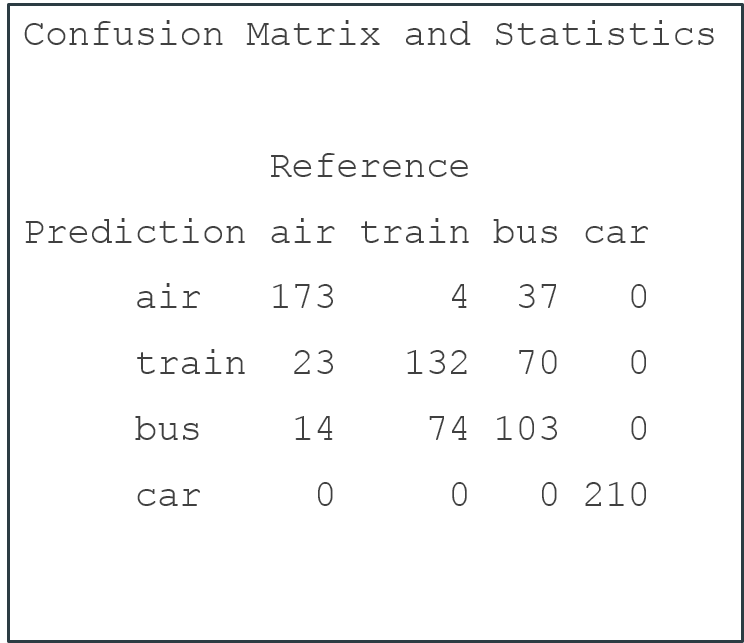
\includegraphics[width=1.06\textwidth]{./img/P11_7}
\end{figure}
\end{minipage}%
\hspace*{3mm}
\begin{minipage}[c]{.6\textwidth}
\begin{figure}
\centering
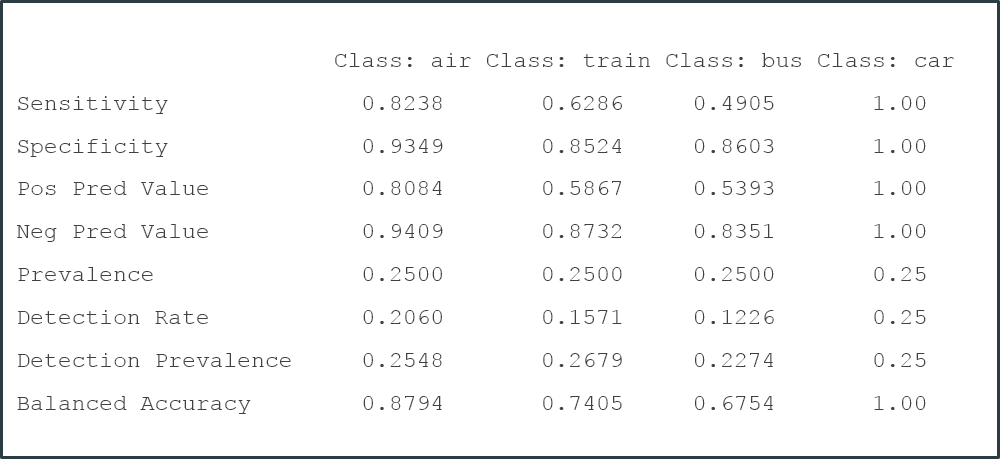
\includegraphics[width=1.06\textwidth]{./img/P11_8}
\end{figure}
\end{minipage}
\end{frame}
%---------------------------------
\subsection{Ordered}
\begin{frame}{MDVs: Ordered responses}
Ordered Logit/Probit models are used to estimate relationships between an ordinal dependent variable and a set of independent variables. \\
\bigskip
An ordinal variable is a variable that is categorical and ordered, for instance, ``poor'', ``good'', and ``excellent''. \\
\bigskip
\underline{\textbf{Ordinal variables – interpretation:}} \\
Say, $y$ is a credit rating on a scale from `0' to `6' (6 is the best rating). Then, credit ratings have ordinal meanings only! \\(6 better than 2)  \\
\smallskip
\textcolor{Blue}{We cannot say that the difference between `4' and `2' is twice as important/prominent as the difference between `6' and `5'}.
\end{frame}
%---------------------------------
\begin{frame}{MDVs: Ordered responses}
\textbf{Ordered Probit model may be derived \\from a latent variable model.} \\
\bigskip
$y^{\ast} = \bm{x \beta} + e, \ e|\bm{x} \sim \textit{Normal}(0,1)$ \\
\bigskip
\underline{Interpretation example:} \\
\medskip
$y_i^{\ast}$ latent variable describing reported health, \\
\smallskip
$\bm{x}_i$ individual health factors.\\
\bigskip
The latent index $y_i^{\ast}$  measures respondent-specific scale of health. This latent scale may differ across individuals $i$ ! \\
\medskip
Once $y_i^{\ast}$ crosses certain - individual-specific - value, respondent report corresponding ``observed'' outcomes, such as:\\
$y_i \in$ \{ bad, poor,  good,  very good,  excellent \}
\end{frame}
%---------------------------------
\begin{frame}{MDVs: Ordered responses}

{\small
\textbf{Ordered Probit Model} \\
\bigskip
\quad $y^{\ast} = \bm{x \beta} + e, \ e|\bm{x} \sim \textit{N}(0,1)$ \\
\bigskip
Observation rules (the relationship between latent and observed $y$): \\
\medskip
\qquad $y_i = 0$ for \hspace*{10mm} $y_i^{\ast} \le \alpha_1$ \\
\medskip
\qquad $y_i = 1$ for \quad  $\alpha_1 < y_i^{\ast} \le \alpha_2$ \\
\medskip
\qquad $y_i = 2$ for \quad  $\alpha_2 < y_i^{\ast} \le \alpha_3$ \\
\qquad \dots \\

\qquad $y_i = J$ for \hspace*{10mm} $y_i^{\ast} > \alpha_J$ \\
\bigskip
where $\bm{x}$ \quad \ regressors, excludes constant (!) \\
\smallskip
\hspace*{9mm} $y$ \quad \ $y_i \in \{0,1,2, \dots, J \} \quad \dots J+1 $ ordered alternatives \\
\smallskip
\hspace*{9mm} $\alpha_j$  \quad unknown (individual) cutpoints/thresholds (ordered);\\ 
\hspace*{17mm} $j = 1, \dots, J$; $\alpha_1 < \alpha_2 < \dots < \alpha_J$ \\
\smallskip
\hspace*{17mm} (\textcolor{Blue}{distances between successive cutpoints may differ})}
\end{frame}
%---------------------------------
\begin{frame}{MDVs: Ordered responses}
Threshold values ($\alpha_1, \alpha_2, \dots, \alpha_J$) are unknown.  We do not know the value of the index necessary to ``push'' someone from reporting \textit{good} to \textit{very good}. \\
\vspace*{6mm}
Threshold values ($\alpha_1, \alpha_2, \dots, \alpha_J$) are different for each individual (at least in theory).\\
\vspace*{6mm}
Ordered Probit/Logit methods not only estimate the vector $\bm{\beta}$, but also the thresholds $\bm{\alpha}$ – i.e. their averages across individuals. \\
\vspace*{6mm}
$P(y=0|\bm{x}) + P(y=1|\bm{x}) + \dots + P(y=J|\bm{x}) = 1$
\end{frame}
%---------------------------------
\begin{frame}{MDVs: Ordered responses}
For Ordered Probit: different outcome probabilities are given as: \\
\bigskip
$P(y=0|\bm{x})=P(\bm{x \beta} + e \le \alpha_1 | \bm{x})=\Phi(\alpha_1 - \bm{x \beta})$ \\
\medskip
$P(y=1|\bm{x})=P(\alpha_1 < \bm{x \beta} + e \le \alpha_2 | \bm{x}) = \Phi(\alpha_2 - \bm{x \beta}) - \Phi(\alpha_1 - \bm{x \beta})$ \\
\medskip
$\vdots$ \\
\medskip
$P(y=J-1|\bm{x}) = \Phi(\alpha_J - \bm{x \beta}) - \Phi(\alpha_{J-1} - \bm{x \beta})$ \\
\medskip
$P(y=J|\bm{x}) = 1 - \Phi(\alpha_J - \bm{x \beta})$ \\
\bigskip
For Ordered Logit, we simply substitute $\Phi(\cdot)$ for the Logistic CDF: $\Lambda (\cdot)$.
\end{frame}
%---------------------------------
\begin{frame}{MDVs: Ordered responses}
MLE is used for estimation. The log-likelihood function for the $i$-th individual (CS unit) is as follows:  \\
\begin{align*}
LL_i (\bm{\alpha, \beta}) & = 1 [y_i = 0] \log[\Phi(\alpha_1 - \bm{x}_i \bm{\beta})] + \\
& + 1[y_i = 1] \log[\Phi(\alpha_2 - \bm{x}_i \bm{\beta}) - \Phi(\alpha_1 - \bm{x}_i \bm{\beta})] + \\
& + \dots + 1[y_i = J] \log[1-\Phi(\alpha_J - \bm{x}_i \bm{\beta})]
\end{align*}
When $J=1$, $P(y=0|\bm{x}) = \Phi(\alpha_1 - \bm{x \beta}) = 1-\Phi(\bm{x \beta} - \alpha_1)$, \\
\smallskip
$P(y=1|\bm{x}) = \Phi(\bm{x \beta} - \alpha_1)$, hence - $\alpha$ is the intercept. 
\end{frame}
%---------------------------------
\begin{frame}{MDVs: Ordered responses}
Interpreting coefficients requires some care: \\
\bigskip
\medskip
\begin{align*}
\frac{\mytikzmark{B1}{\partial p_0(\bm{x})}}{\partial x_k} & = -\beta_k \phi(\alpha_1 - \bm{x \beta}), ~~~ \frac{p_J(\bm{x})}{\partial x_k} =\mytikzmark{B2}{\beta_k \phi (\alpha_J - \bm{x \beta})} \\
\frac{\partial p_j(\bm{x})}{\partial x_k} & = \mytikzmark{B3}{\beta_k[\phi(\alpha_{j-1} - \bm{x \beta}) - \phi(\alpha_j - \bm{x \beta})]}
\end{align*} \\
\bigskip
For a small change in $x_k$, the sign of the resulting effect on\\
\smallskip
$P(y=0|\bm{x})$ and \\
\smallskip
$P(y=J|\bm{x})$ \\
\smallskip
is unambiguously determined by the sign of  $\beta_k$.
\begin{tikzpicture}[<-,overlay,remember picture,inner sep=1pt,shorten <=0.2em,font=\footnotesize]
\tikzset{
    mynode/.style={rectangle, draw=Red, minimum size=0.5cm, text width=5cm},
    myarrow/.style={->, >=stealth, semithick, Red}
}
\node[mynode] at (-6.4,5.5)(box1){$p_0 = P(y=0|\bm{x})$; i.e. expression describes the change in $P$ of the ``worst'' outcome};
\draw[myarrow] (box1) --++ (B1);
\node[mynode] at (0.35,5.5)(box2){change in $P$ of the ``best'' outcome};
\draw[myarrow] (box2) --++ (B2);
\node[mynode] at (-2.65,2.6)(box3){change in $P$ of an intermediate outcome $j$};
\draw[myarrow] (box3) --++ (B3);
\end{tikzpicture}
\end{frame}
%---------------------------------
\begin{frame}{MDVs: Ordered responses}
Interpreting coefficients requires some care: 
\begin{align*}
\frac{\partial p_0(\bm{x})}{\partial x_k} & = -\beta_k \phi(\alpha_1 - \bm{x \beta}), ~~~ \frac{p_J(\bm{x})}{\partial x_k} = \beta_k \phi (\alpha_J - \bm{x \beta}) \\
\frac{\partial p_j(\bm{x})}{\partial x_k} & = \mytikzmark{B}{\beta_k[\phi(\alpha_{j-1} - \bm{x \beta}) - \phi(\alpha_j - \bm{x \beta})]}
\end{align*} \\
\bigskip
\medskip
For a small change in $x_k$, the sign of the resulting effect on\\
\medskip
$P(y=j|\bm{x})$ is ambiguous, it depends on the ratio of \\
\medskip
$|\alpha_{j-1} - \bm{x \beta}|$ vs. $|\alpha_j - \bm{x \beta}|$ 
\smallskip
\\ \dots (remember, $\phi (\cdot)$  is symmetric around zero).
\begin{tikzpicture}[<-,overlay,remember picture,inner sep=1pt,shorten <=0.2em,font=\footnotesize]
\tikzset{
    mynode/.style={rectangle, draw=Red, minimum size=0.5cm, text width=5cm},
    myarrow/.style={->, >=stealth, semithick, Red}
}
\node[mynode] at (-5.05,2.7)(box){change in $P$ of a given intermediate outcome $j$};
\draw[myarrow] (box) --++ (B);
\end{tikzpicture}
\end{frame}
%---------------------------------
\begin{frame}{MDVs: Ordered responses}
Interpreting coefficients: 
\begin{align*}
\frac{\partial p_0(\bm{x})}{\partial x_k} & = -\beta_k \phi(\alpha_1 - \bm{x \beta}), ~~~ \frac{p_J(\bm{x})}{\partial x_k} = \beta_k \phi (\alpha_J - \bm{x \beta}) \\
\frac{\partial p_j(\bm{x})}{\partial x_k} & = \beta_k[\phi(\alpha_{j-1} - \bm{x \beta}) - \phi(\alpha_j - \bm{x \beta})]
\end{align*} \\
\medskip
\underline{Example:}\\
\medskip
For 3 ordered outcomes, $y_i \in \{0,1,2\}$, we have $\beta_k >0$. Then:
\begin{align*}
\partial p_0(\bm{x}) & / \partial x_k < 0, \\
\partial p_2(\bm{x}) & / \partial x_k > 0, \\
\partial p_1(\bm{x}) & / \partial x_k \ \textnormal{can have either positive or negative sign.}
\end{align*} 
\end{frame}
%---------------------------------
\begin{frame}{MDVs: Ordered responses}
In ordered Probit/Logit estimation, $\hat{\bm{\beta}}$ coefficients are usually of limited interest (have limited interpretation). \\
\medskip
Instead, we are interested in response probabilities $P(y=j|\bm{x})$ \\
\medskip
As in other nonlinear models, we can compute and interpret PEAs or APEs. (Bootstrap standard errors) \\
\medskip
Confusion matrix may be used for prediction (classification) accuracy evaluation. \\
\medskip
Many generalizations and extension to ordered models are possible. For example, it makes sense to work with ``cumulative'' probabilities of ``at least'' or ``at best'' defined outcomes: \\
\medskip
$P(y \le j|\bm{x}) = P(y^{\ast} \le a_j|\bm{x}) = G(a_j - \bm{x \beta})$, \ $j = 0,1, \dots, J-1$
\end{frame}
%---------------------------------
\section{Other LDVs}
\subsection{Corner solution response data: Tobit model}
\begin{frame}{Corner solution response data: Tobit model}
The Tobit model for corner solution responses
\begin{itemize}
\item Corner solution response (many zero outcomes + roughly continuous positive outcomes).
\item In many economic contexts, decision problems are such that either a positive amount or a zero amount is chosen (e.g. demand for alcohol)
\item A linear regression model may be inadequate in such cases as predictions may be negative and effects of explanatory variables are linear
\item The Tobit model makes use of a latent variable formulation
\end{itemize}
\bigskip
Definition of the Tobit model \\
\medskip
$y^{\ast} = \bm{x \beta} + u$, \ $u|\bm{x} \sim \mytikzmark{1}{N(0, \sigma^2)}$\\
$y = \max \mytikzmark{2}{(0,y^{\ast})}$
\begin{tikzpicture}[<-,overlay,remember picture,inner sep=1pt,shorten <=0.2em,font=\scriptsize]
\tikzset{
    mynode/.style={rectangle, minimum size=0.5cm, text width=5cm},
    myarrow/.style={->, >=stealth, semithick, Red}
}
\node[mynode] at (5.3,1.4)(box1){Conditional on the values of the explanatory variables, the error term is homoscedastic normally distributed};
\draw[myarrow] (box1) --++ (1);
\node[mynode] at (5,0.11)(box2){The observed outcome of the dependent variable is positive or zero};
\draw[myarrow] (box2) --++ (2);
\end{tikzpicture}
\end{frame}
%---------------------------------
\begin{frame}{Corner solution response data: Tobit model}
\underline{\textbf{Maximum likelihood estimation of the Tobit model}}
\begin{align*}
f(y_i|\bm{x}_i; \bm{\beta}, \sigma) = 
  \begin{cases}
   \mytikzmark{A}{(2 \pi \sigma^2)^{-\frac{1}{2}} \exp[-(y_i - \bm{x}_i \bm{\beta})^2 / (2 \sigma^2)]} & \ \text{if } y_i > 0 \\
  \mytikzmark{B}{1 - \Phi(\bm{x}_i \bm{\beta} / \sigma)}  & \ \text{if } y_i = 0 \\
  \end{cases}
\end{align*} \\
\vspace*{1.4cm}
\underline{Maximization of the log-likelihood:} \\
\medskip
$\max LL(\bm{\beta}, \sigma) = \sum \limits_{i=1}^{n} \log f(y_i|\bm{x}_i; \bm{\beta}, \sigma) \to \hat{\beta}_0, \hat{\beta}_1, \dots, \hat{\beta}_k, \hat{\sigma}$ \\
\medskip
{\footnotesize
As in the Logit/Probit case, the maximization problem is highly nonlinear. It cannot be solved analytically and has to be solved with the help of computer software using e.g. Newton-Raphson methods.}
\begin{tikzpicture}[<-,overlay,remember picture,inner sep=1pt,shorten <=0.2em,font=\footnotesize]
\tikzset{
    mynode/.style={rectangle, minimum size=0.5cm, text width=10.7cm},
    myarrow/.style={->, >=stealth, semithick, Red}
}
\node[mynode] at (-2.9,3.9)(box){For positive outcomes, the normal density (applied to $y_i - \bm{x}_i \bm{\beta}$) is used, for zero outcomes the probability is one minus the probability that the latent variable is greater than zero (see Probit).};
\draw[myarrow] (box) --++ (A);
\draw[myarrow] (box) --++ (B);
\end{tikzpicture}
\end{frame}
%---------------------------------
\begin{frame}{Corner solution response data: Tobit model}
\underline{\textbf{Interpretation of the coefficients in the Tobit model}} \\
\bigskip
\underline{Conditional mean for all outcomes:}
\begin{flalign*}
E(y|\bm{x}) & = P(y > 0|\bm{x}) \cdot E(y|y>0,\bm{x}) + P(y = 0|\bm{x}) \cdot 0 = && \\
& = \mytikzmark{one}{\boxed{\Phi(\bm{x \beta}/ \sigma) \cdot E(y|y>0,\bm{x})}} &&
\end{flalign*} \\
\vspace*{1cm}
\underline{Conditional mean for positive outcomes:}\\
\medskip
$E(y|y>0,\bm{x}) = \bm{x \beta} + \mytikzmark{two}{\boxed{\sigma \lambda(\bm{x \beta}/\sigma)}}$ \\
\medskip
$\lambda(c) = \phi(c)/\Phi(c) > \mytikzmark{three}{0}$ \\
\begin{tikzpicture}[<-,overlay,remember picture,inner sep=1pt,shorten <=0.2em,font=\scriptsize]
\tikzset{
    mynode/.style={rectangle, minimum size=0.5cm, text width=4.8cm},
    myarrow/.style={->, >=stealth, semithick, Red}
}
\node[mynode] at (9,3.25)(box1){The mean for all outcomes is a scaled version of the mean for only the positve outcomes (this is the reason why a regression using only the positive outcomes would yield wrong results)};
\draw[myarrow] (box1) --++ (one);
\node[mynode] at (9,0.8)(box2){The mean for only the positive outcomes is the usual linear regression but plus an extra term (this is again a reason why an ordinary linear regression would yield wrong results)};
\draw[myarrow] (box2) --++ (two);
\node[mynode] at (6,-0.1)(box3){This is the so called \underline{inverse Mills ratio}};
\draw[myarrow] (box3) --++ (three);
\end{tikzpicture}
\end{frame}
%---------------------------------
\begin{frame}{Corner solution response data: Tobit model}
\underline{\textbf{Partial effects of interest in the Tobit model}} \\
\bigskip
\underline{On the probability of a nonzero outcome:} \\
\medskip
$\frac{\partial P(y > 0| \bm{x})}{\partial x_j} = \mytikzmark{a}{(\beta_j / \sigma) \phi (\bm{x \beta}/\sigma)}$ \\
\vspace*{1cm}
\underline{On the mean of positive outcomes:}\\
\medskip
$\frac{\partial E(y|y>0,\bm{x})}{\partial x_j} = \beta_j \overbrace{\{ 1 - \lambda(\bm{x \beta}/\sigma)[\bm{x \beta}/\sigma + \lambda(\bm{x \beta}/\sigma)] \}}^{\mytikzmark{b}{}}$ \\
\bigskip
\underline{On the mean of all possible outcomes including zero:} \\
\medskip
$\frac{\partial E(y|\bm{x})}{\partial x_j} = \mytikzmark{c}{\beta_j \Phi(\bm{x \beta}/\sigma)}$ \\
\begin{tikzpicture}[<-,overlay,remember picture,inner sep=1pt,shorten <=0.2em,font=\scriptsize]
\tikzset{
    mynode/.style={rectangle, minimum size=0.5cm, text width=4.8cm},
    myarrow/.style={->, >=stealth, semithick, Red}
}
\node[mynode] at (8,4.8)(box1){Note that all partial effects depend on the explanatory variables and the error variance};
\draw[myarrow] (box1) --++ (a);
\node[mynode] at (9.1,3.3)(box2){This adjustment factor can be shown to lie between zero and one};
\draw[myarrow] (box2) --++ (b);
\node[mynode] at (7,0.6)(box3){Note that this adjustment factor also lies between zero and one};
\draw[myarrow] (box3) --++ (c);
\end{tikzpicture}
\end{frame}
%---------------------------------
\begin{frame}{Corner solution response data: Tobit model}
\underline{\textbf{Estimation of average partial effects in the Tobit model}} \\
\bigskip
\underline{APE on the probability of a nonzero outcome:} \\
\medskip
$\hat{\textnormal{APE}}_{1,j} = \mytikzmark{a}{n^{-1} \sum \limits_{i=1}^{n} (\hat{\beta}_j / \hat{\sigma}) \phi (\bm{x}_i \hat{\bm{\beta}} / \hat{\sigma})}$ \\
\vspace*{1cm}
\underline{APE on the mean of positive outcomes:}\\
\medskip
$\hat{\textnormal{APE}}_{2,j} = n^{-1} \sum \limits_{i=1}^{n} \hat{\beta}_j \{ 1 - \lambda(\bm{x}_i \hat{\bm{\beta}} / \hat{\sigma}) [\bm{x}_i \hat{\bm{\beta}} / \hat{\sigma} + \mytikzmark{b}{\lambda(\bm{x}_i \hat{\bm{\beta}} / \hat{\sigma})}] \}$ \\
\bigskip
\underline{APE on the mean of all possible outcomes including zero:} \\
\medskip
$\hat{\textnormal{APE}}_{3,j} = n^{-1} \sum \limits_{i=1}^{n} \hat{\beta}_j \Phi (\bm{x}_i \hat{\bm{\beta}} / \mytikzmark{c}{\hat{\sigma}})$ \\
\begin{tikzpicture}[<-,overlay,remember picture,inner sep=1pt,shorten <=0.2em,font=\scriptsize]
\tikzset{
    mynode/.style={rectangle, minimum size=0.5cm, text width=4.8cm},
    myarrow/.style={->, >=stealth, thin, Red}
}
\node[mynode] at (9,4.7)(box){Analogous formulas are available for partial effects at the average (PEA) but they have the aforementioned disadvantages};
\draw[myarrow] (box) --++ (a);
\draw[myarrow] (box) --++ (b);
\draw[myarrow] (box) --++ (c);
\end{tikzpicture}
\end{frame}
%---------------------------------
\begin{frame}{Corner solution response data: Tobit model}

{\footnotesize
\underline{\textbf{Specification and other advanced topics in Tobit/Logit/Probit models}} \\
\begin{itemize}
\item \textcolor{Blue}{In the Tobit model, regressors influence the values of observed positive outcomes and the probability of positive outcome observations at the same time.}\\
\medskip
\item This may be unrealistic in many cases, for example, when modeling the relationship between the amount of life insurance and person's age.\\
\medskip
\item For such cases, more advanced so-called \underline{hurdle models} can be used.
\item As in Logit/Probit models, heteroscedasticity may arise in Tobit.\\
\medskip
\item ML estimates may be wrong if distributional assumptions do not hold.\\
\medskip
\item There are methods to deal with endogeneity in Logit/Probit/Tobit.\\
\medskip
\item Logit/Probit/Tobit models are available for panel/time series data.
\end{itemize}}
\end{frame}
%---------------------------------
\begin{frame}{Corner solution response data: Tobit model}

{\small \underline{\textbf{Tobit example: Annual hours worked by married women}}}
\begin{minipage}[t]{.48\textwidth}
\vspace*{4mm}
\begin{table}[]
\resizebox{\textwidth}{!}{%
\begin{tabular}{lcc}
\hline
\multicolumn{3}{c}{\textbf{Dependent Variable: \textit{hours}}}                                                                           \\ \hline
\textbf{\begin{tabular}[c]{@{}l@{}}Independent\\ Variables\end{tabular}} & \textbf{Linear (OLS)}           & \textbf{Tobit (MLE)}           \\ \hline
\textit{nwifeinc}                                                        & $\underset{(2.54)}{-3.45}$      & $\underset{(4.46)}{-8.81}$     \\ \hline
\textit{educ}                                                            & $\underset{(12.95)}{28.76}$     & $\underset{(21.58)}{80.65}$    \\ \hline
\textit{exper}                                                           & $\underset{(9.96)}{65.67}$      & $\underset{(17.28)}{131.56}$   \\ \hline
\textit{exper$^2$}                                                       & $\underset{(.325)}{-.700}$      & $\underset{(0.54)}{-1.86}$     \\ \hline
\textit{age}                                                             & $\underset{(4.36)}{-30.51}$     & $\underset{(7.42)}{-54.41}$    \\ \hline
\textit{kidslt6}                                                         & $\underset{(58.85)}{-442.09}$   & $\underset{(111.88)}{-894.02}$ \\ \hline
\textit{kidsge6}                                                         & $\underset{(23.18)}{-32.78}$    & $\underset{(38.64)}{-16.22}$   \\ \hline
\textit{constant}                                                        & $\underset{(270.78)}{1,330.48}$ & $\underset{(446.44)}{965.31}$  \\ \hline
\begin{tabular}[c]{@{}l@{}}Log-likelihood\\ value\end{tabular}           & -                               & -3,819.09                      \\ 
$R$-squared                                                              & .266                            & .274                           \\ 
$\hat{\sigma}$                                                           & 750.18                          & 1,122.02                       \\ \hline
\end{tabular}%
}
\end{table}
\end{minipage}
\hspace*{0.1mm}
\begin{minipage}[t]{.48\textwidth}
{\scriptsize
Because of the different scaling factors involved, Tobit coefficients are not comparable to OLS coefficients.\\

To compare Tobit and OLS, one has to compare average partial effects (or partial effects at the average). It turns out that partial effects of Tobit and OLS are different in a number of cases.\\

Another difference between Tobit and OLS is that, due to the linearity of the model, OLS assumes constant partial effects, whereas partial effects are nonconstant in Tobit.\\

In the given example, OLS yields negative predictions of hours worked for 39 out of 753 women. This is not much but it may be a reason to view the linear model as misspecified.\\

}
\end{minipage}
\end{frame}
%---------------------------------
\subsection{Censored data: Censored data models}
\begin{frame}{Censored data: Censored data models}
\textbf{Censored data/models} (response variable is censored above and/or below some threshold; random sampling holds). \\
\medskip
Often, dependent variable is censored in the sense that values are only reported up to a certain level (e.g. top coded wealth).\\
\medskip
\underline{Censored normal regression model:}\\
\begin{align*}
\mytikzmark{1}{\circledd{$y_i$}} & = \bm{x}_i \bm{\beta} + u_i, \ u_i|\bm{x}_i,c_i \sim N(0,\sigma^2) \\
\vspace{0.3cm}
\mytikzmark{2}{\circledd{$w_i$}} & = \mytikzmark{3}{\min (y_i, c_i)}
\end{align*} \\
\medskip
Regressing $y_i$ on $x_i$ $\Rightarrow$ correct results; but $y_i$ is unobserved.\\
\medskip
Regressing $w_i$ on $x_i$ will yield incorrect results (even if only the uncensored observations are used in this regression).
\begin{tikzpicture}[<-,overlay,remember picture,inner sep=1pt,shorten <=0.2em,font=\scriptsize]
\tikzset{
    mynode/.style={rectangle, minimum size=0.05cm, text width=4cm},
    mynode2/.style={rectangle, minimum size=0.05cm, text width=3cm},
    myarrow/.style={->, >=stealth, semithick, Red}
}
\node[mynode] at (-7,3.8)(box1){True outcome (unobserved)};
\draw[myarrow] (box1) --++ (1);
\node[mynode2] at (-7.5,3)(box2){Observed outcome};
\draw[myarrow] (box2) --++ (2);
\tikzset{
    mynode/.style={rectangle, draw=Red, minimum size=0.5cm, text width=4cm},
    myarrow/.style={->, >=stealth, semithick, Red}
}
\node[mynode] at (-1,2.2)(box3){If the true outcome exceeds the censoring threshold, only the threshold is reported};
\draw[myarrow] (box3) --++ (3);
\end{tikzpicture}
\end{frame}
%---------------------------------
\begin{frame}{Censored data: Censored data models}
\textbf{ML estimation of the censored regression model}\\
\bigskip
$P(w_i = c_i|\bm{x}_i) = P(y_i \ge c_i|\bm{x}_i) = $ \\
\smallskip
$ = P(u_i \ge c_i - \bm{x}_i \bm{\beta}) = 1-\Phi[(c_i - \bm{x}_i \bm{\beta})/\sigma] $ \\
\bigskip
Probability/density function of observed outcome conditional on explanatory variables:
\begin{align*}
f(w_i|\bm{x}_i; \bm{\beta}, \sigma) =
\begin{cases}
(2 \pi \sigma^2)^{- \frac{1}{2}} \exp [-(w_i - \bm{x}_i \bm{\beta})^2 / (2 \sigma^2)] & \ \text{if } \mytikzmark{1}{w_i} < c_i \\
1 - \Phi((c_i - \bm{x}_i \bm{\beta})/\sigma) & \ \text{if } w_i = c_i
\end{cases} 
\end{align*} 
\underline{Maximization of log-likelihood:} \\
$\max LL(\bm{\beta}, \sigma) = \sum \limits_{i=1}^{n} \log f(w_i|\bm{x}_i, c_i) \ \to \ \hat{\beta}_0, \hat{\beta}_1, \dots, \hat{\beta}_k, \hat{\sigma}$
\begin{tikzpicture}[<-,overlay,remember picture,inner sep=1.2pt,shorten <=0.2em,font=\scriptsize]
\tikzset{
    mynode/.style={rectangle, draw=Red, minimum size=0.5cm, text width=5.4cm},
    myarrow/.style={->, >=stealth, thin, Red}
}
\node[mynode] at (-0.8,3)(box){If the censoring threshold does not bind, the density of the outcome is normal};
\draw[myarrow] (box) --++ (1);
\end{tikzpicture}
\end{frame}
%---------------------------------
\begin{frame}{Censored data: Censored data models}

{\footnotesize \textbf{Censored regression example: estimation of criminal recidivism}}

\begin{table}[]
\hspace*{-6.5cm}
\noindent\makebox[\textwidth]{%
\tiny
\begin{tabular}{lc}
\hline
\multicolumn{2}{c}{\mytikzmark{XA}{\textbf{Dependent Variable: $\log (\textit{durat})$}}}                                                                                       \\ \hline
\textbf{\begin{tabular}[c]{@{}l@{}}Independent\\ Variables\end{tabular}}      & \textbf{\begin{tabular}[c]{@{}c@{}}Coefficient \\ (Standard Error)\end{tabular}} \\ \hline
\textit{workprg}                                                              & $\underset{(.120)}{-.063}$                                                       \\ \hline
\textit{priors}                                                               & $\underset{(.021)}{-.137}$                                                       \\ \hline
\textit{tserved}                                                              & \mytikzmark{XB}{\circledd{$\underset{(.003)}{-.019}$}}                                                       \\ \hline
\textit{felon}                                                                & $\underset{(.145)}{.444}$                                                        \\ \hline
\textit{alcohol}                                                              & $\underset{(.144)}{-.635}$                                                       \\ \hline
\textit{drugs}                                                                & $\underset{(.133)}{-.298}$                                                       \\ \hline
\textit{black}                                                                & $\underset{(.117)}{-.543}$                                                       \\ \hline
\textit{married}                                                              & $\underset{(.140)}{.341}$                                                        \\ \hline
\textit{educ}                                                                 & $\underset{(.025)}{.023}$                                                        \\ \hline
\textit{age}                                                                  & $\underset{(.0006)}{.0039}$                                                      \\ \hline
\textit{constant}                                                             & $\underset{(.348)}{4.099}$                                  \\ 
\hline
\begin{tabular}[c]{@{}l@{}}Log-likelihood \\ value $\hat{\sigma}$\end{tabular} & \begin{tabular}[c]{@{}c@{}}-1,597.06\\ 1.810\end{tabular}                        \\ \hline
\end{tabular}}
\end{table}

\begin{tikzpicture}[<-,overlay,remember picture,inner sep=1.2pt,shorten <=0.2em,font=\scriptsize]
\tikzset{
    mynode/.style={rectangle, minimum size=0.5cm, text width=6.7cm},
    myarrow/.style={->, >=stealth, thin, Red}
}
\node[mynode] at (8.4,5.9)(boxA){The variable \textit{durat} measures the time in months until a prison inmate is arrested after being released from prison. Of 1,445 inmates, 893 had not been arrested during the time they were followed. Their time out of prison is censored (because a follow-up project ended, if there were some later arrests, they were not observed).};
\draw[myarrow] (boxA) --++ (XA);
	\node[mynode] at (8.4,3.9)(boxB){For example, if the time in prison was one month longer, this 		reduced the expected duration until the next arrest by about 1.9 \%.};
	\draw[myarrow] (boxB) --++ (XB);
		\node[mynode] at (8.4,1.8)(box){\textcolor{Blue}{\underline{In the censored regression 				model, the coefficients}} \textcolor{Blue}{\underline{can be directly interpreted.}} This is 		contrary to the Tobit model (coefficients cannot be directly interpreted). The censored 				regression model and the Tobit 	model have a similar structure, but in the Tobit model, the 		outcome is of a nonlinear nature whereas in the censored regression model, the outcome 			is linear but incompletely observed.};
\end{tikzpicture}
\end{frame}
%---------------------------------
\subsection{Truncated data, Heckit}
\begin{frame}{Truncated data}
\begin{itemize}
\item Truncated data/regression models (for some observations, response variable is missing due to non-random selection)
\item In a truncated regression model, the outcome and the explanatory variables are only observed if the outcome is less or equal some value $c_i$
\item In this case, the sample is not a random sample from the population (because some units will never be a part of the sample)
\item \underline{Truncated normal regression model:}
\end{itemize}
\vspace*{-2mm}
\begin{flalign*}
y_i = \bm{x}_i \bm{\beta} + u_i, \ u_i|\bm{x}_i \sim N(0, \sigma^2) \\
(y_i, \bm{x}_i) \ \textnormal{\underline{only observed if}} \ y_i \le c_i
\end{flalign*}
\vspace*{-4mm}
\begin{itemize}
\item OLS would not yield correct results: \\ MLR.2 (random sampling) is violated
\end{itemize}
\begin{tikzpicture}[<-,overlay,remember picture,inner sep=0pt,shorten <=0.2em,font=\scriptsize]
\tikzset{
    mynode/.style={rectangle, very thick, draw=Red, dashed, minimum size=1.35cm, text width=5.7cm},
}
\node[mynode] at (5.5,2.5)(box){};
\end{tikzpicture}
\end{frame}
%---------------------------------
\begin{frame}{Truncated data}
\textbf{ML estimation of the truncated regression model} \\
\bigskip
Density of an observed outcome conditional on explanatory variables and the threshold $c_i$ \\
\bigskip
$g(y_i|\bm{x}_i, c_i) = \frac{f(y_i|\bm{x}_i \bm{\beta}, \sigma^2)}{P(y_i \le c_i|\bm{x}_i)} = \frac{\mytikzmark{1}{f(y_i|\bm{x}_i \bm{\beta}, \sigma^2)}}{\mytikzmark{2}{F(c_i|\bm{x}_i \bm{\beta}, \sigma^2)}}$ \\
\bigskip
\underline{Likelihood maximization:} \\
\bigskip
$\max LL(\bm{\beta}, \sigma) = \sum \limits_{i=1}^{n} \log g(y_i|\bm{x}_i, c_i) \ \to \ \hat{\beta}_0, \hat{\beta}_1, \dots, \hat{\beta}_k, \hat{\sigma}$ \\
\bigskip
As in the censored regression model, nonnormality \\or heteroscedasticity in the truncated regression model lead \\to inconsistency. 
\begin{tikzpicture}[<-,overlay,remember picture,inner sep=0.6pt,shorten <=0.2em,font=\scriptsize]
\tikzset{
    mynode/.style={rectangle, draw=White, minimum size=1cm, text width=4.0cm},
    myarrow/.style={->, >=stealth, semithick, Red}
}
\node[mynode] at (6.8,4.2)(box){Density and distribution \\function of a normal distribution with mean $\bm{x}_i \bm{\beta}$ and \\variance $\sigma^2$};
\draw[myarrow] (box) -- ++ (1);
\draw[myarrow] (box) -- ++ (2);
\end{tikzpicture}
\end{frame}
%---------------------------------
\begin{frame}{Truncated data}
\textbf{\underline{Sample selection corrections}}\\
\begin{itemize}
\item[] The question is under which assumptions a sample with nonrandom sample selection can be used to infer relationships in the population
\end{itemize}
\textbf{When is OLS on the selected sample consistent?}\\
\medskip
$y = \bm{x\beta} + u, \ E(u|\bm{x})=\mytikzmark{0}{0}$ \\
\medskip
\mytikzmark{si}{\circled{$s_i$}} \\
\medskip
$s_i y_i = s_i \bm{x}_i \bm{\beta} + \mytikzmark{R}{s_i u_i}$\\
\bigskip
\underline{Condition for consistency of OLS:} \\ $E(su)=0$\\$E[(sx_j)(su)] = E(sx_ju) = 0$ (because $s^2=s$ as $s$ is binary)
\begin{tikzpicture}[<-,overlay,remember picture,inner sep=0.6pt,shorten <=0.2em,font=\scriptsize]
\tikzset{
    mynode/.style={rectangle, minimum size=1cm, text width=6cm},
    myarrow/.style={->, >=stealth, semithick, Red}
}
\node[mynode] at (1.8,3.3)(box1){Population model};
\draw[myarrow] (box1) -- ++ (0);
	\node[mynode] at (-0.5,2.3)(box2){Sample selection indicator, $s_i=1$\\ if observation selected/included in \\the sample, $s_i=0$ otherwise};
	\draw[myarrow] (box2) -- ++ (si);
		\node[mynode] at (1,1.49)(box3){Regression based \\on the selected sample};
		\draw[myarrow] (box3) -- ++ (R);
\end{tikzpicture}
\end{frame}
%---------------------------------
\begin{frame}{Truncated data}

{\small
Unbiasedness: $E(u|x_1,x_2,\dots,x_k)=0$ vs. $E(su|sx_1,sx_2,\dots,sx_k)=0$\\
\medskip
\textbf{Conditions for OLS consistency on the selected sample:} \\
\begin{itemize}
\item[1.] $s$ is independent of explanatory variables and the error term.\\$E(sx_ju)=E(s)E(x_ju) = 0$ because $E(x_ju) = 0$.
\item[2.] $s$ is completely determined by explanatory variables. $sx_j = f(\bm{x})$. Hence, corr($sx_j,u$) = 0 and $E(su|sx_1,sx_2,\dots,sx_k)=0$
\item[3.] $s$ depends on the explanatory variables and other factors that are uncorrelated with the error term.
\end{itemize}
\textbf{Similar conditions apply to IV/2SLS estimation}
\begin{itemize}
\item[] Besides explanatory variables $\bm{x}$, conditions extend to the full set of IVs: $\bm{z}$ as well.
\end{itemize}
\textbf{Sample selection and nonlinear models estimated by ML}
\begin{itemize}
\item[] MLE (probit, logit) produces consisten etstimates if $s$ is fully determined by regressors (cond. 2.).
\end{itemize}}
\end{frame}
%---------------------------------
\begin{frame}{Truncated data (non-random selection): Heckit model}

{\footnotesize
\textbf{Incidental truncation (Heckman model)}
\begin{itemize}
\item[] Special case of nonrandom selection: regressors are always observed, but the observation of the dependent variable is non-random (the same variables that determine the outcome of $y_i$ also determine whether it is observed).
\end{itemize}
\bigskip
\textbf{Example: Wage offer function using a sample of working women}
\begin{itemize}
\item We are interested in the wage a woman with certain characteristics would be offered on the labor market if she decided to work.\\
\medskip
\item Unfortunately, we only observe the wages of women who actually work, i.e. who have accepted the wage offered to them. The sample is truncated because women who do not work (but who would be offered a wage if they asked for it) are never in the sample.\\
\medskip
\item Truncation of this kind is called incidental truncation because $y_i$ observation depends on another variable (here: labor force participation).
\end{itemize}}
\end{frame}
%---------------------------------
\begin{frame}{Truncated data (non-random selection): Heckit model}
\textbf{Definition of Heckman model}
\begin{flalign*}
& y = \bm{x \beta} + \mytikzmark{u}{u} && \\
& s = \mytikzmark{s}{1[\bm{z} \bm{\gamma} + v \ge 0]} && \\
& (u, v) | \bm{x}, \bm{z} \sim \mytikzmark{N}{N(0,\sigma^2),~\rho} &&
\end{flalign*}
\textbf{Selection bias in OLS} \\
\bigskip
$E(y|\bm{x}, \bm{z}, s = 1) = \bm{x \beta} + \mytikzmark{B}{\boxed{\rho \lambda (\bm{z} \bm{\gamma})}}$

\begin{tikzpicture}[<-,overlay,remember picture,inner sep=0.6pt,shorten <=0.2em,font=\scriptsize]
\tikzset{
    mynode/.style={rectangle, minimum size=1cm, text width=6cm},
    myarrow/.style={->, >=stealth, semithick, Red}
}
\node[mynode] at (5.5,3.5)(box1){Main equation (e.g. wage equation)};
\draw[myarrow] (box1) -- ++ (u);
	\node[mynode] at (6.7,3)(box2){Selection equation (e.g. whether working)};
	\draw[myarrow] (box2) -- ++ (s);
		\node[mynode] at (8,2)(box3){The error terms of both equations are jointly normally distributed (independent of the explanatory variables) with correlation coefficient $\rho$};
		\draw[myarrow] (box3) -- ++ (N);
			\node[mynode] at (8.7,0)(box4){For example, if the correlation of unobserved wage 					determinants and unobserved determinants of the work decision is positive, the 						women observed working will have higher wages than expected from their 								characteristics (= positive selection)};
			\node[mynode] at (3,-0.5)(box5){Running the regression on the truncated sample 						suffers from omitted variable bias};
			\draw[myarrow] (box4) -- ++ (B);
			\draw[myarrow] (box5) -- ++ (B);
\end{tikzpicture}
\end{frame}
%---------------------------------
\begin{frame}{Truncated data (non-random selection): Heckit model}
\textbf{Estimation of Heckman model}\\ 
\bigskip
\underline{1) Estimation of correction term:}
\begin{flalign*}
& P(s=1|\bm{z}) = \Phi \mytikzmark{1}{(\bm{z} \bm{\gamma})} && \\
& \hat{\lambda} = \phi(\bm{z} \hat{\bm{\gamma}}) / \Phi \mytikzmark{2}{(\bm{z} \hat{\bm{\gamma}})} && 
\end{flalign*}
\underline{2) Include estimated correction term in regression:}\\
\medskip
$y_i = \beta_0 + \beta_1 x_{i1} + \dots + \beta_k x_{ik} + \mytikzmark{3}{\circled{$\rho$}}\mytikzmark{4}{\hat{\lambda}_i} + \textit{error}$
\begin{tikzpicture}[<-,overlay,remember picture,inner sep=0.6pt,shorten <=0.2em,font=\scriptsize]
\tikzset{
    mynode/.style={rectangle, minimum size=1cm, text width=6cm},
    myarrow/.style={->, >=stealth, semithick, Red}
}
\node[mynode] at (0,2.4)(box1){Estimate Probit for work decision using all observations (working and nonworking women)};
\draw[myarrow] (box1) -- ++ (1);
	\node[mynode] at (0,1.45)(box2){Calculate inverse Mills ratio using Probit \\coefficients (only $\hat{\lambda}_i$ for $s_i=1$ are necessary)};
	\draw[myarrow] (box2) -- ++ (2);
		\node[mynode] at (-5,-1)(box3){If this coefficient is different from zero, there is 						nonignorable sample selection bias};
		\draw[myarrow] (box3) -- ++ (3);
			\node[mynode] at (1,-1.1)(box4){There have to be explanatory variables in the 						selection equation that are not in the main equation (exclusion restrictions), otherwise 				there is multicollinearity because the inverse Mills ratio is almost linear in $z$};
			\draw[myarrow] (box4) -- ++ (4);
\end{tikzpicture}
\end{frame}
%---------------------------------
\begin{frame}{Truncated data (non-random selection): Heckit model}
\textbf{Heckit example: Wage offer for married women} 
\begin{table}[]
\hspace*{-5cm}
\begin{tabular}{lcc}
\hline
\multicolumn{3}{c}{\textbf{Dependent Variable: $\log (\textit{wage})$}}                                                                                                          \\ \hline
\textbf{\begin{tabular}[c]{@{}l@{}}Independent\\ Variables\end{tabular}} & \textbf{OLS}                                       & \textbf{Heckit}                                    \\ \hline
\textit{educ}                                                            & $\underset{(.014)}{.108}$                          &  $\mytikzmark{1}{\underset{(.016)}{.109}}$                      \\ \hline
\textit{exper}                                                           & $\underset{(.012)}{.042}$                          & $\underset{(.016)}{.044}$                          \\ \hline
\textit{exper}$^2$                                                       & $\underset{(.00039)}{-.00081}$                     & $\underset{(.00044)}{-.00086}$                     \\ \hline
\textit{constant}                                                        & $\underset{(.199}{-.522}$                          & $\underset{(.307)}{-.578}$                         \\ \hline
$\hat{\lambda}$                                                          & -                                                  &  \mytikzmark{2}{\circledd{$\underset{(.134)}{.032}$}}                          \\ \hline
\begin{tabular}[c]{@{}l@{}}Sample size\\ $R$-squared\end{tabular}        & \begin{tabular}[c]{@{}c@{}}428\\ .157\end{tabular} & \begin{tabular}[c]{@{}c@{}}428\\ .157\end{tabular} \\ \hline
\end{tabular}
\end{table}
\begin{tikzpicture}[<-,overlay,remember picture,inner sep=0.6pt,shorten <=0.2em,font=\scriptsize]
\tikzset{
    mynode/.style={rectangle, minimum size=1cm, text width=4cm},
    myarrow/.style={->, >=stealth, semithick, Red}
}
\node[mynode] at (9,4.7)(box1){The standard errors of the two-step Heckman method are actually wrong and have to be corrected (not done here). One can also use a maximum likelihood procedure.};
\draw[myarrow] (box1) -- ++ (1);
	\node[mynode] at (9,1.7)(box2){There is no significant sample selection bias. This is the reason why OLS and Heckman estimates are so similar.};
	\draw[myarrow] (box2) -- ++ (2);
\end{tikzpicture}
\end{frame}
%%---------------------------------
\end{document}